%
% Switches
%
% Aleph Objects Firewall
%
% Copyright (C) 2014, 2015, 2016 Aleph Objects, Inc.
%
% This document is licensed under the Creative Commons Attribution 4.0
% International Public License (CC BY-SA 4.0) by Aleph Objects, Inc.
%

\section{Overview}
There are free software solutions for network switches, allegedly. Lets see.


Currently, the network is using 1 gig-e basically everywhere, except phones
which are 100M (and so is anything plugged into them). The Internet backbone
connection is 500M fiber, plus unlicensed wifi. An additional 1 gig backbone
connection to another provider is being evaluated.


We need a few hundred gig-e ports, with 10 gig uplinks using SFP+ fiber.
Around six 48-port switches, plus more if we add co-location.


\section{Free Software for Network Switches}

\subsection{ONIE}
\begin{figure}[h!]
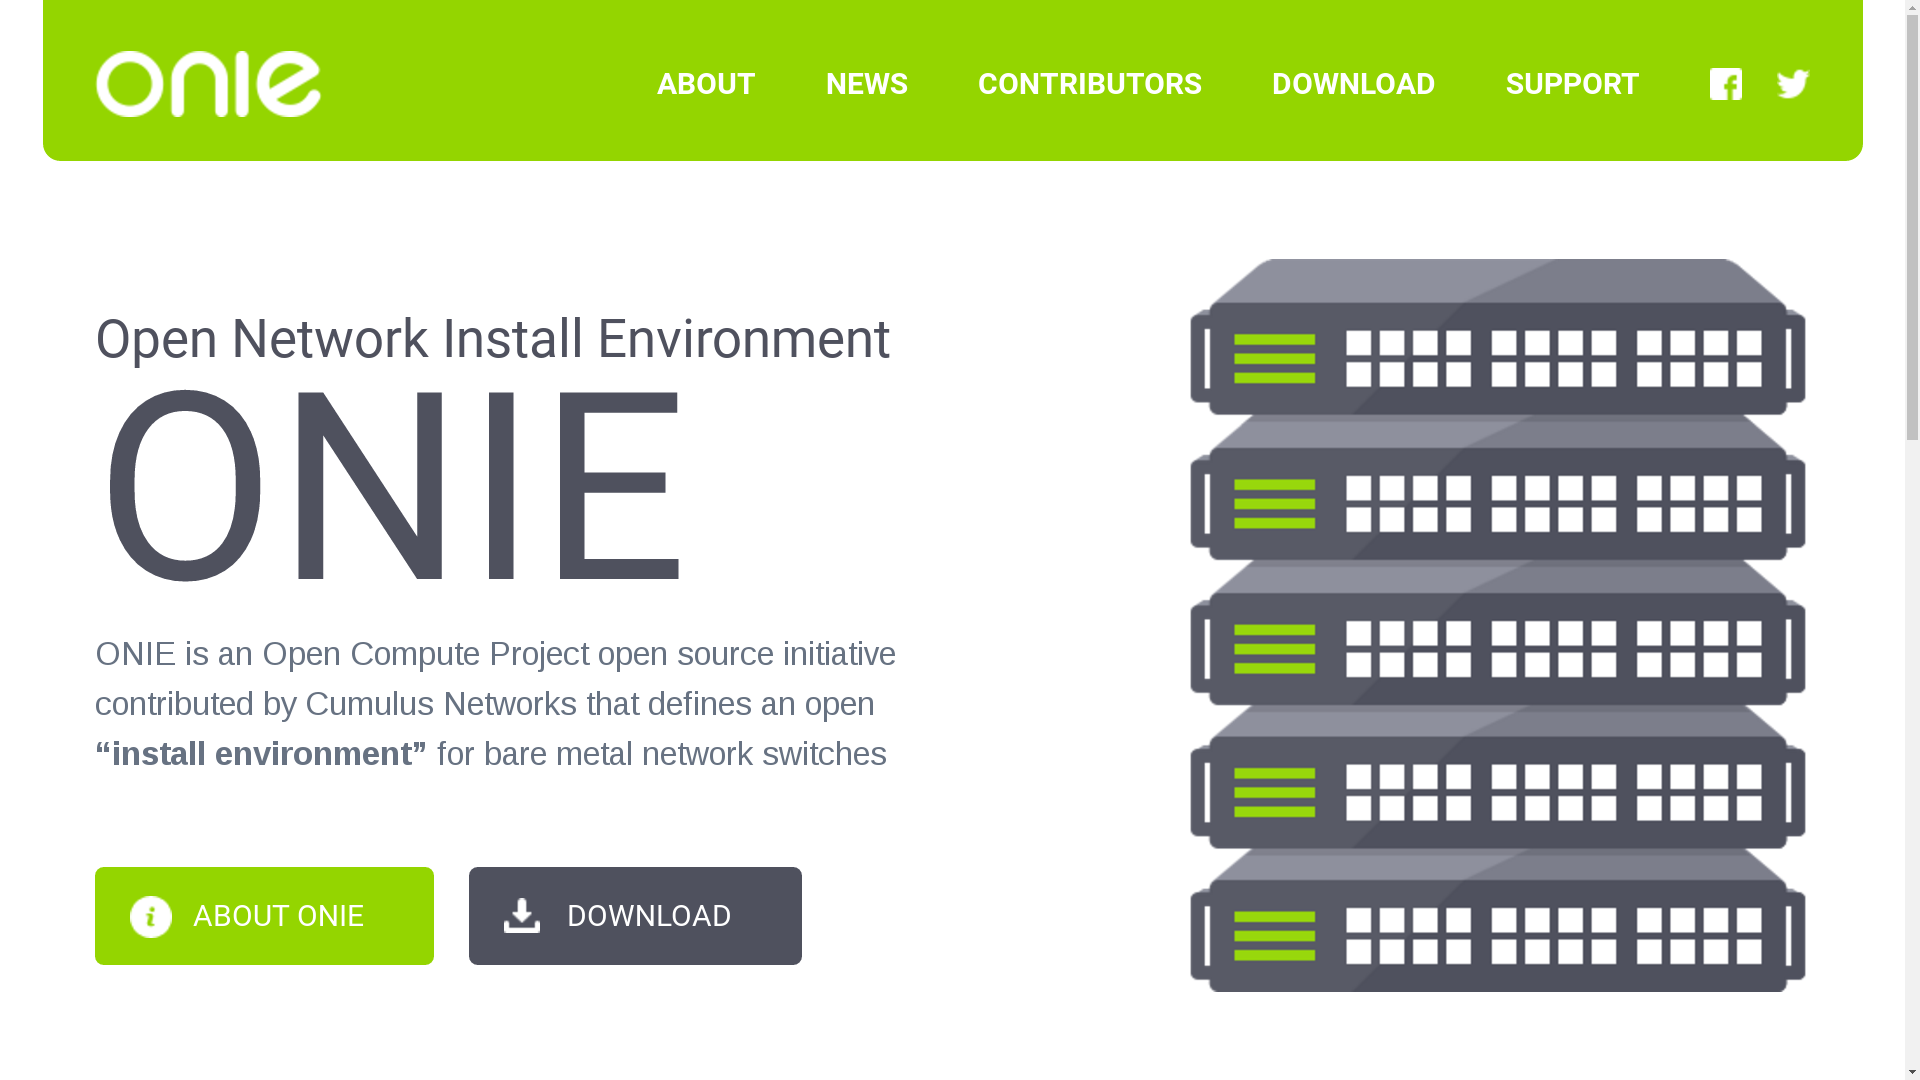
\includegraphics[keepaspectratio=true,height=1.10\textheight,width=1.00\textwidth,angle=0]{www-onie.png}
 \caption{ONIE Website}
 \label{fig:www-onie}
\end{figure}


\begin{itemize}
 \item Website: \\ \url{http://onie.org}
 \item Source code: \\ \url{https://github.com/opencomputeproject/onie}
 \item Wiki: \\ \url{https://github.com/opencomputeproject/onie/wiki}
 \item License: GPLv2
 \item Hardware status: \\ \url{http://www.opencompute.org/wiki/Networking/ONIE/HW_Status}
 \item Operating System Support: \\ \url{http://www.opencompute.org/wiki/Networking/ONIE/NOS_Status}
\end{itemize}

``The Open Network Install Environment (ONIE) is an Open Compute Project open source initiative driven by a community to define an open ``install environment'' for bare metal network switches, such as existing ODM switches and the upcoming OCP Network Switch design. ONIE enables a bare metal network switch ecosystem where end users have a choice among different network operating systems.... ONIE was contributed to the Open Compute Project.... ONIE is an open source ``install environment'', that acts as an enhanced boot loader utilizing facilities in a Linux/BusyBox environment. This small Linux operating system allows end-users and channel partners to install the target network OS as part of data center provisioning, in the fashion that servers are provisioned.''


\subsection{Open Network Linux}
\begin{figure}[h!]
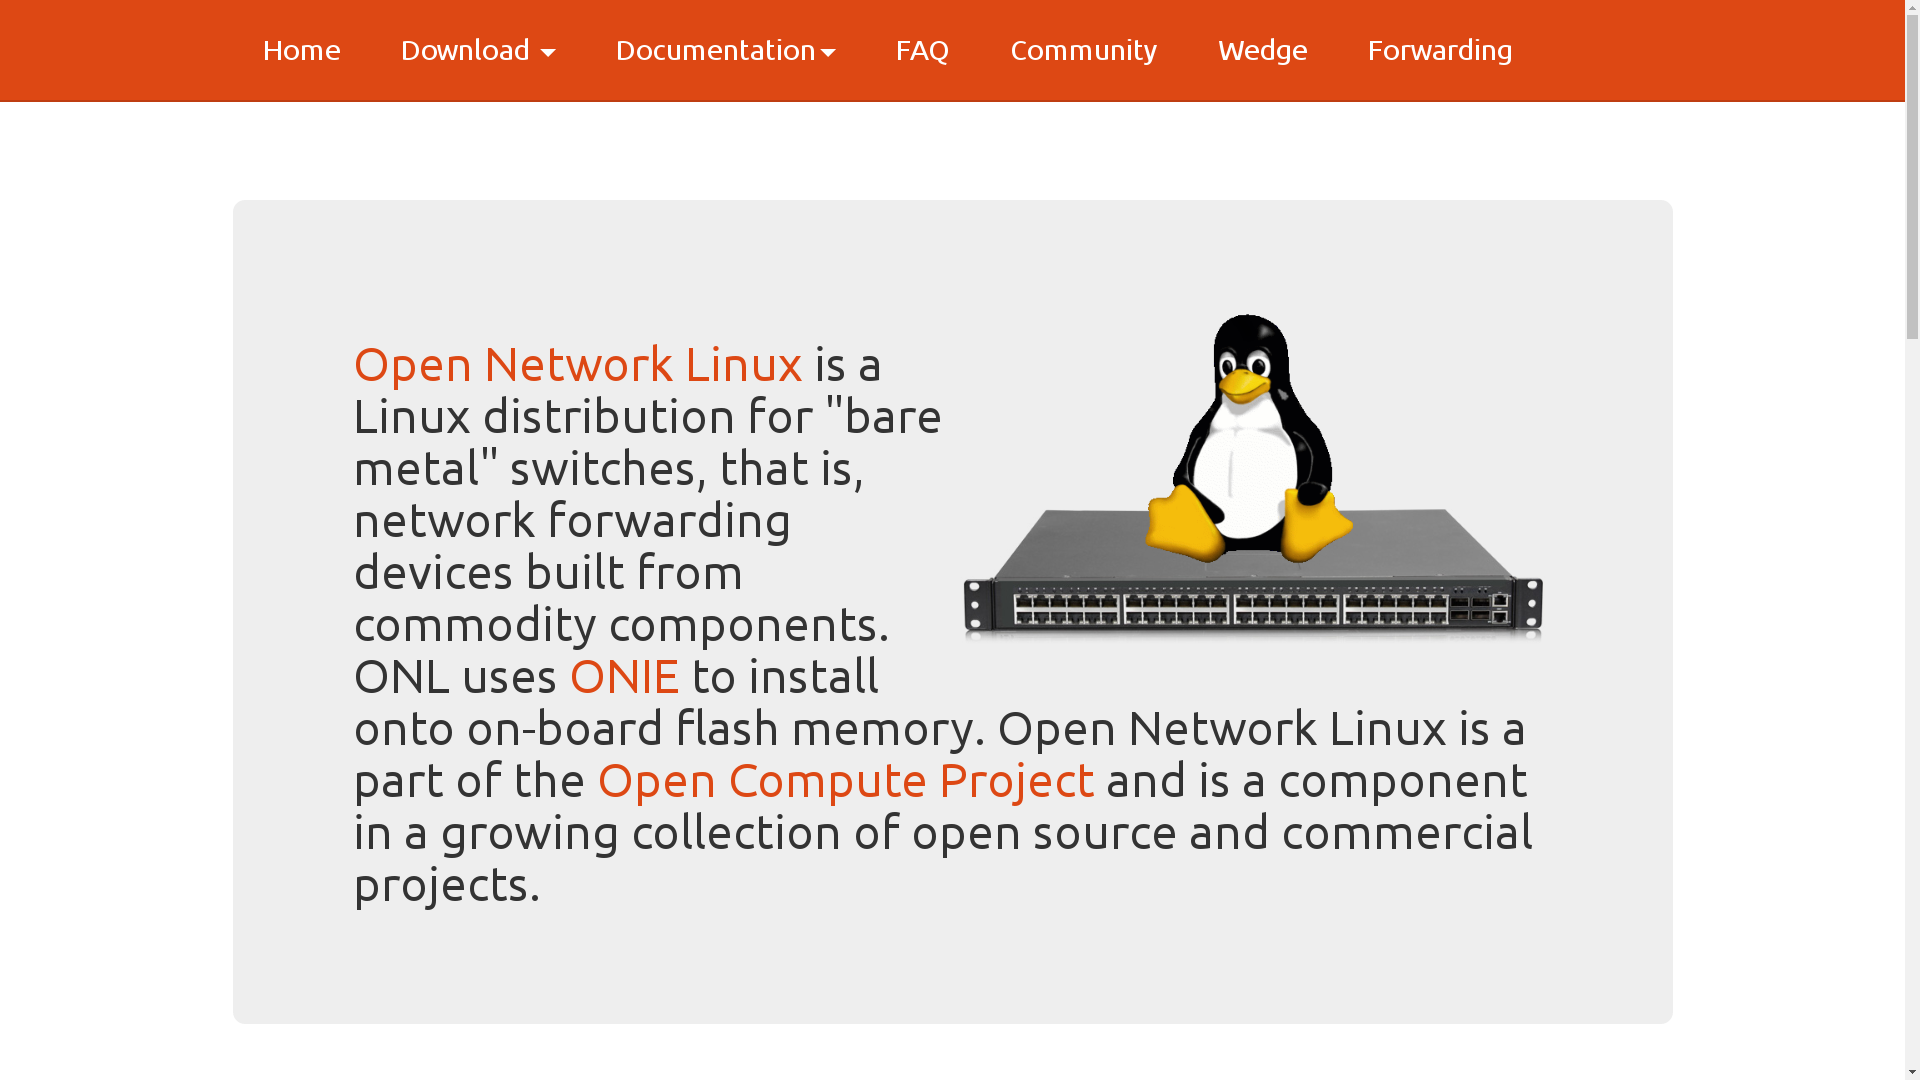
\includegraphics[keepaspectratio=true,height=1.10\textheight,width=1.00\textwidth,angle=0]{www-onl.png}
 \caption{Open Network Linux Website}
 \label{fig:www-onl}
\end{figure}


\begin{itemize}
 \item Website: \\ \url{https://opennetlinux.org/}
\end{itemize}


Distro for bare metal switches.


This is probably what we'll use. We'll see.


``Open Network Linux is a Linux distribution for "bare metal" switches, that is, network forwarding devices built from commodity components. ONL uses ONIE to install onto on-board flash memory. Open Network Linux is a part of the Open Compute Project and is a component in a growing collection of open source and commercial projects.''


Supports these switch fabric APIs:
\begin{itemize}
 \item OF-DPA
 \item OpenNSL --- May be non-free Broadcom.
 \item SAI
\end{itemize}


Forwarding Agents:
\begin{itemize}
 \item \url{http://www.quagga.net/}{Quagga} ---
       ``BGP4, BGP4+, OSPFv2, OSPFv3, IS-IS, RIPv1, RIPv2, and RIPng''. In Debian.
 \item \url{http://bird.network.cz/}{BIRD} ---
       ``Internet routing daemon with full support for all the major routing protocols.'' In Debian.
 \item Facebook FBOSS --- Open Source for Facebook scale.
 \item Azure SONiC --- ``SONiC is an open source project for network routers and switches''
\end{itemize}


\subsection{Snaproute}
\begin{figure}[h!]
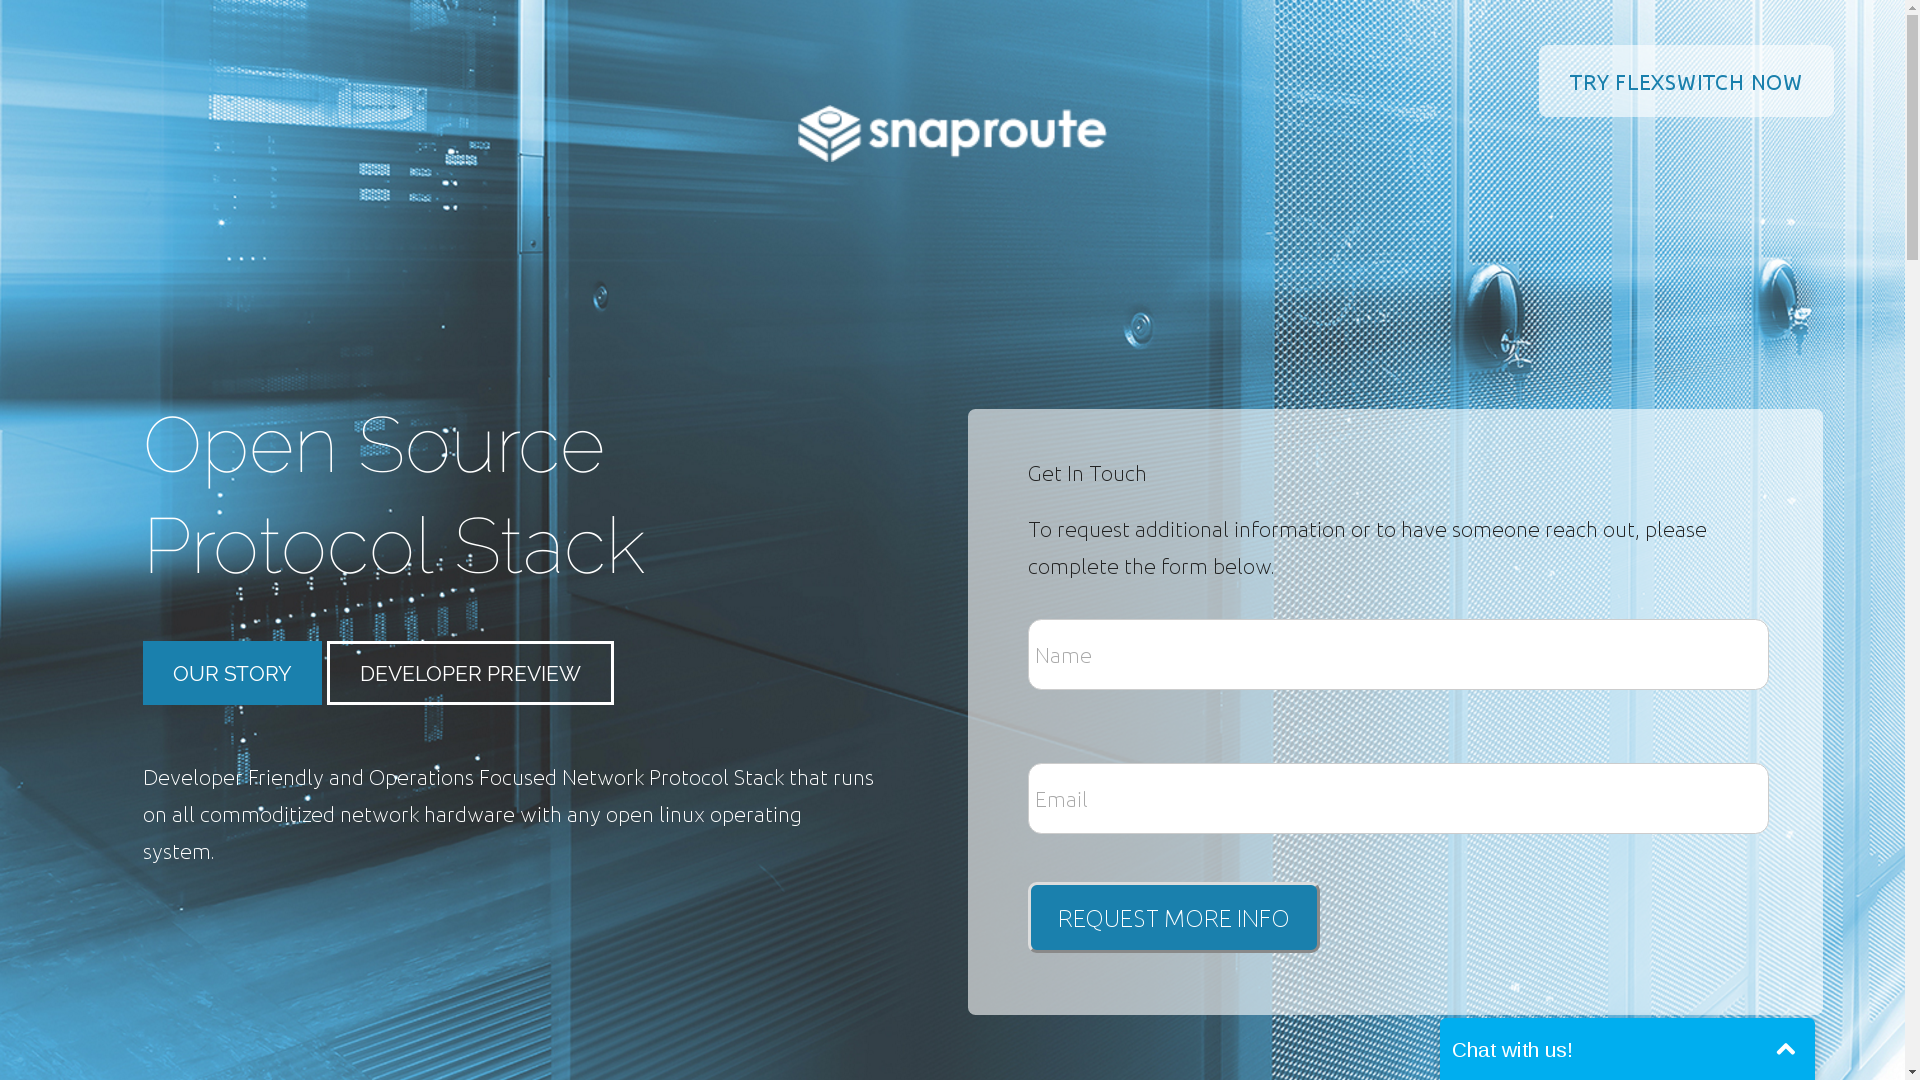
\includegraphics[keepaspectratio=true,height=1.10\textheight,width=1.00\textwidth,angle=0]{www-snaproute.png}
 \caption{Snaproute Website}
 \label{fig:www-snaproute}
\end{figure}


\begin{itemize}
 \item aka OpenSnaproute, FlexSwitch.
 \item Website: \\ \url{http://www.snaproute.com/}
 \item Documentation: \\ \url{https://opensnaproute.github.io/docs/}
 \item Written in Go programming language.
\end{itemize}


``Open source network stack for enterprise...
Developer Friendly and Operations Focused Network Protocol Stack that runs on
all commoditized network hardware with any open linux operating system.''


\subsection{OpenSwitch}
\begin{figure}[h!]
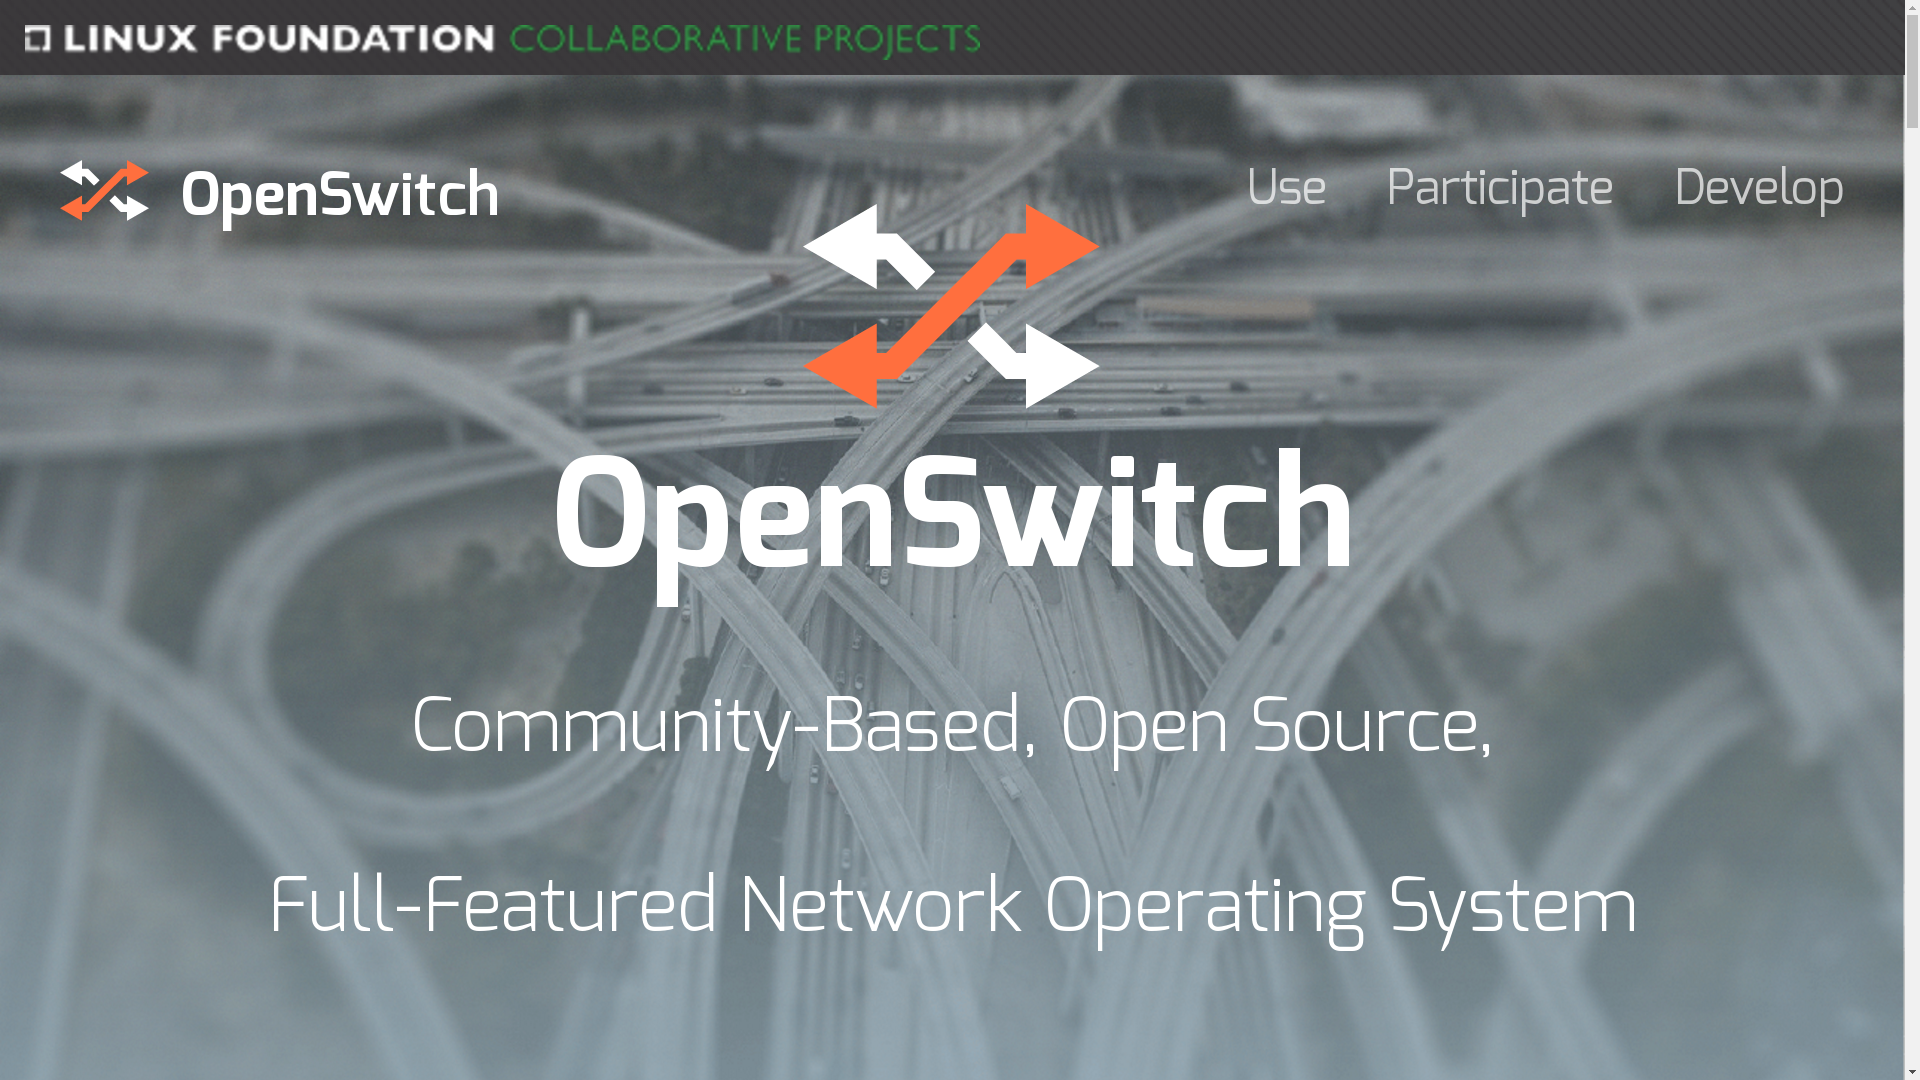
\includegraphics[keepaspectratio=true,height=1.10\textheight,width=1.00\textwidth,angle=0]{www-openswitch.png}
 \caption{OpenSwitch Website}
 \label{fig:www-openswitch}
\end{figure}


\begin{itemize}
 \item Website: \\ \url{http://www.openswitch.net/}
 \item Linux Foundation project. Other big names.
 \item Hardware Compatibility (spoiler: Broadcom): \\ \url{http://www.openswitch.net/documents/user/hardware-compatibility}
\end{itemize}


``Community-Based, Open Source, Full-Featured Network Operating System.''


The hardware compatibilty list has Broadcom based systems from HPE Altoline
and Edge-Core. All 10Gig+, high-end gear.


\subsection{FBOSS}
\begin{figure}[h!]
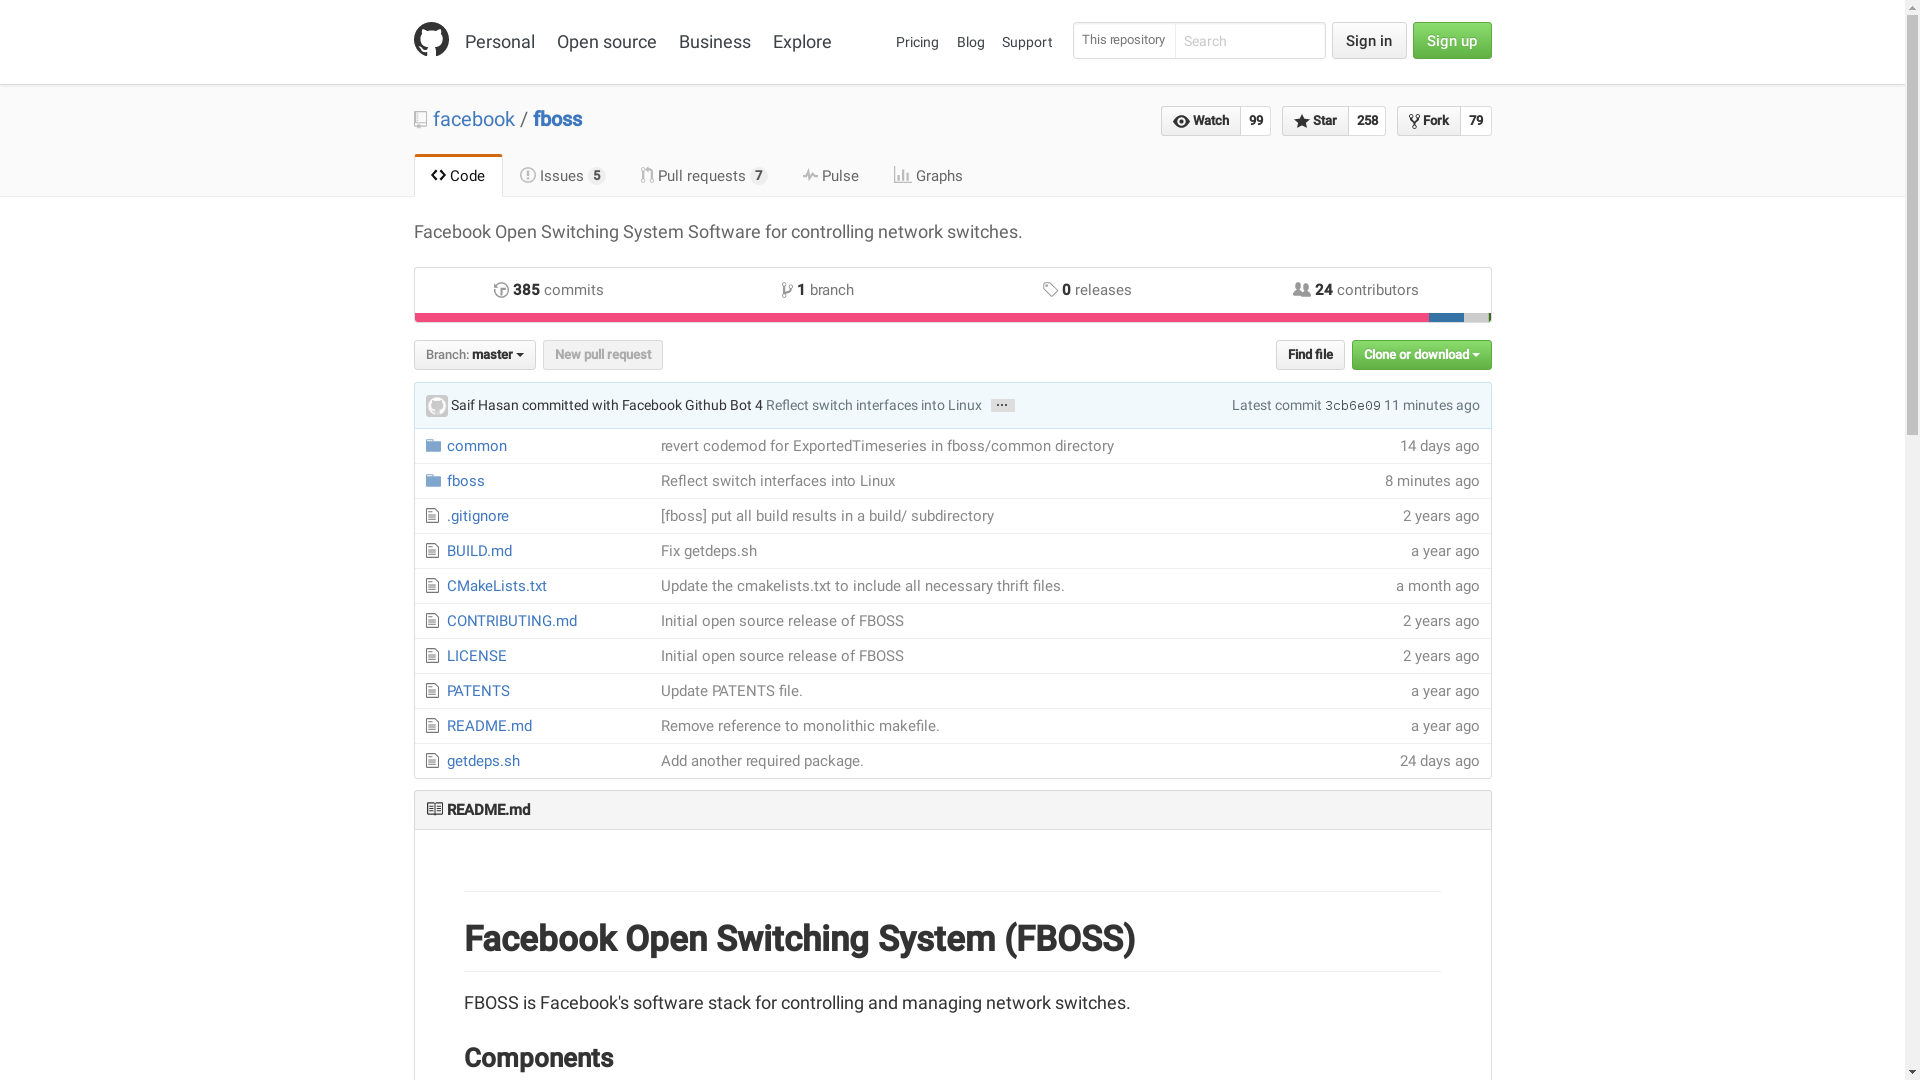
\includegraphics[keepaspectratio=true,height=1.10\textheight,width=1.00\textwidth,angle=0]{www-fboss.png}
 \caption{FBOSS Website}
 \label{fig:www-fboss}
\end{figure}


\begin{itemize}
 \item Website: \\ \url{https://github.com/facebook/fboss}
 \item Source code: \\ \url{https://github.com/facebook/fboss}
 \item License: ``BSD''
\end{itemize}


``Facebook Open Switching System (FBOSS).
FBOSS is Facebook's software stack for controlling and managing network switches.''


I am guessing this is going to be way overkill. Nom.


\subsection{Open Compute Project}
\begin{figure}[h!]
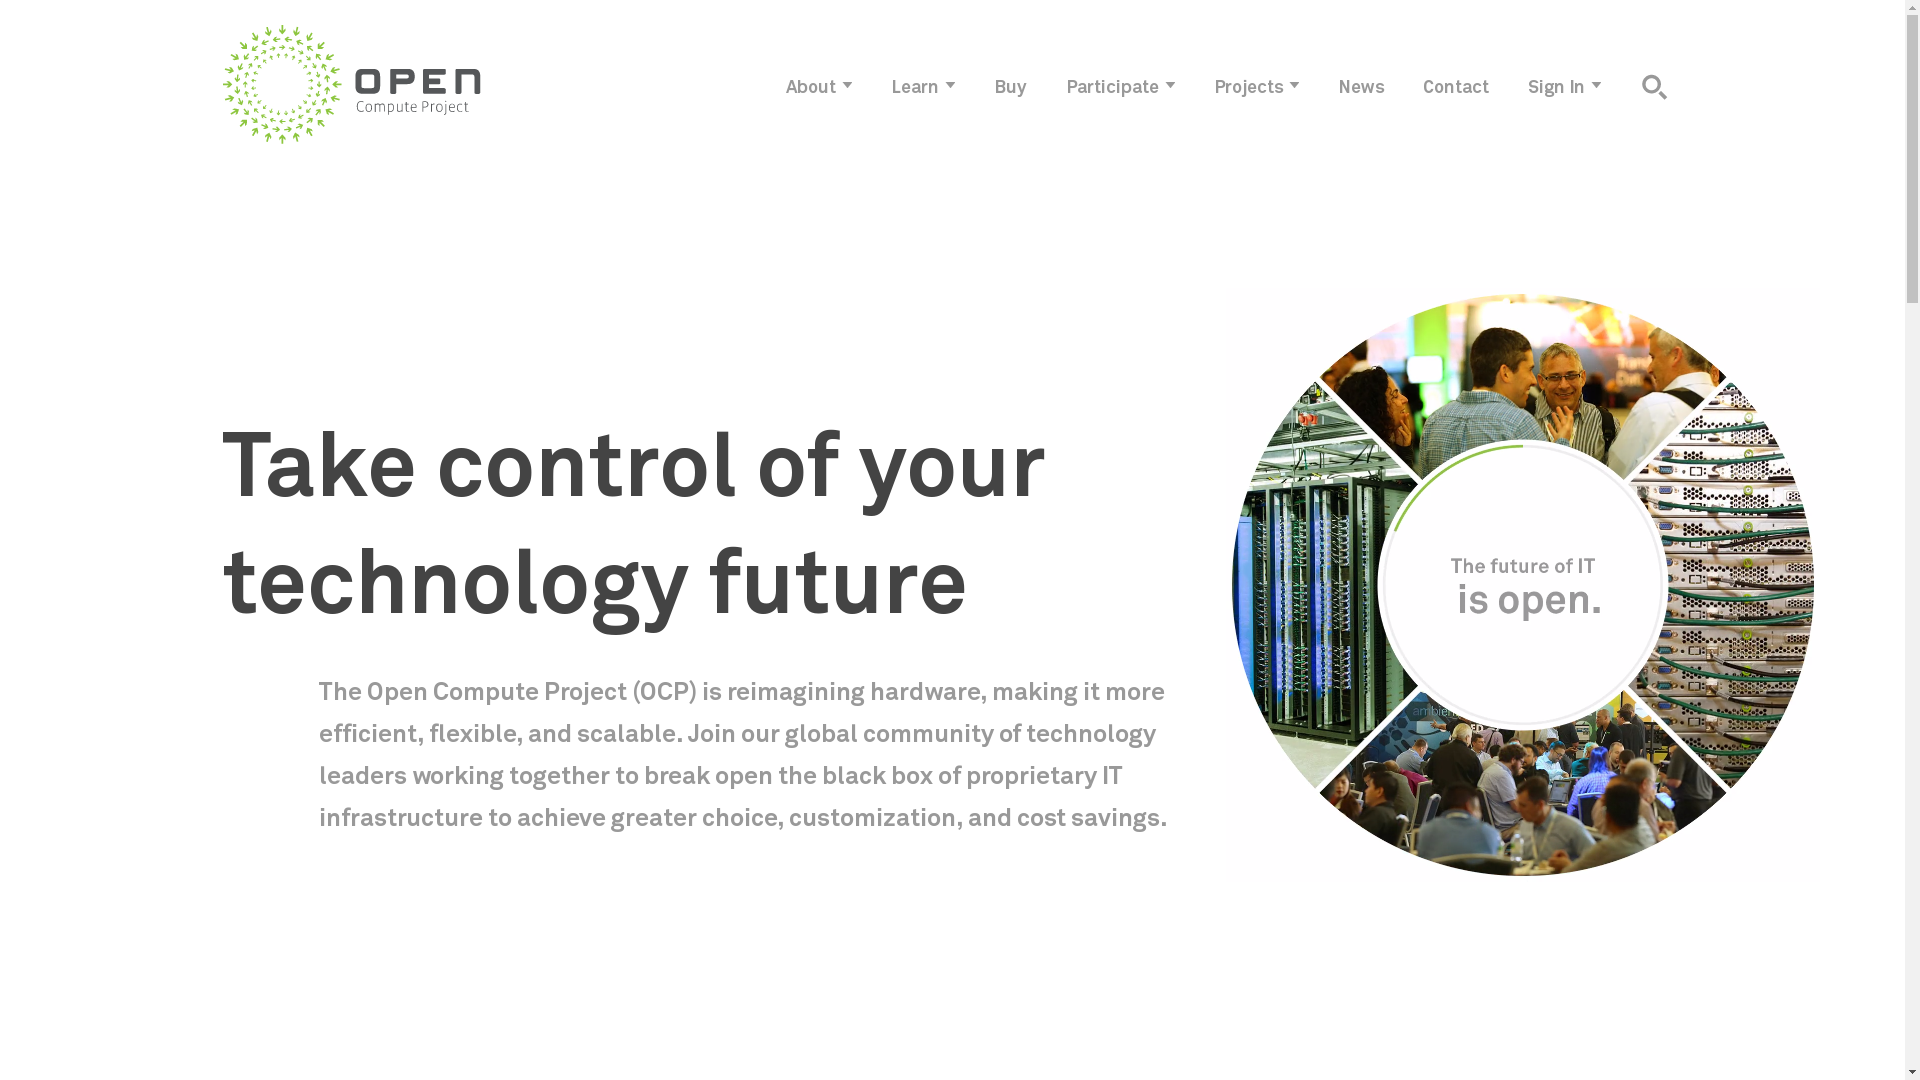
\includegraphics[keepaspectratio=true,height=1.10\textheight,width=1.00\textwidth,angle=0]{www-opencompute.png}
 \caption{OpenCompute Website}
 \label{fig:www-opencompute}
\end{figure}


\begin{itemize}
 \item \url{http://www.opencompute.org/}
 \item \url{http://github.com/opencomputeproject}
\end{itemize}

``The Open Compute Project (OCP) is a collaborative community focused on redesigning hardware technology to efficiently support the growing demands on compute infrastructure.''


Project so massive data centers can be more ``open'' and interoperate better
between vendors, by using free software. Started by Facebook, supported by
Google and others that run huge datacenters.


Although it is supposed to be an ``Open Source'' project, it includes non-free
parts.


\subsection{OpenDataPlane}
\begin{figure}[h!]
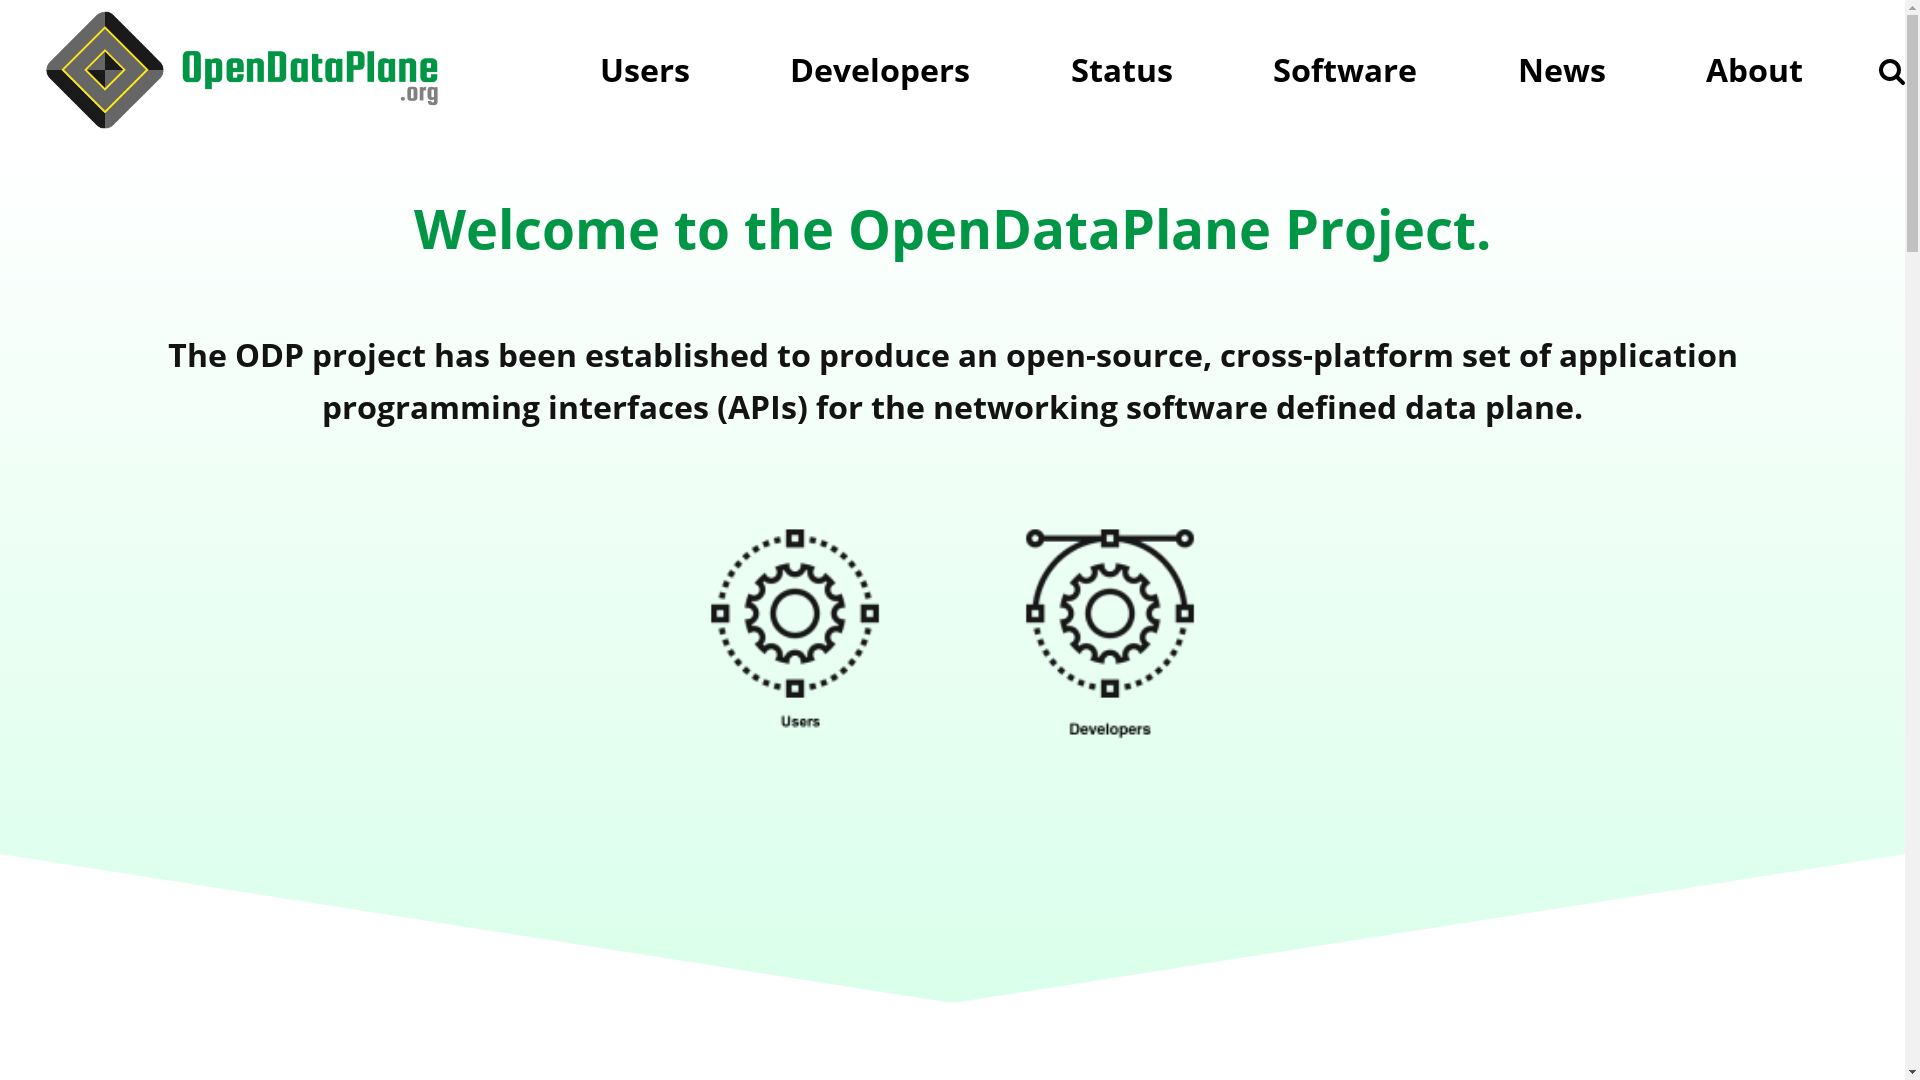
\includegraphics[keepaspectratio=true,height=1.10\textheight,width=1.00\textwidth,angle=0]{www-opendataplane.png}
 \caption{OpenDataPlane Website}
 \label{fig:www-opendataplane}
\end{figure}


\begin{itemize}
 \item Website: \\ \url{http://opendataplane.org/}
 \item Debian Apt Repository: \\ \url{http://deb.opendataplane.org/}
\end{itemize}

``The ODP project has been established to produce an open-source, cross-platform set of application programming interfaces (APIs) for the networking software defined data plane.''


These can run on top of ODP:

\begin{itemize}
 \item OpenFastPath \\ \url{http://www.openfastpath.org/}
 \item Open vSwitch \\ \url{http://openvswitch.org/}
\end{itemize}


\subsection{OpenFastPath}
\begin{figure}[h!]
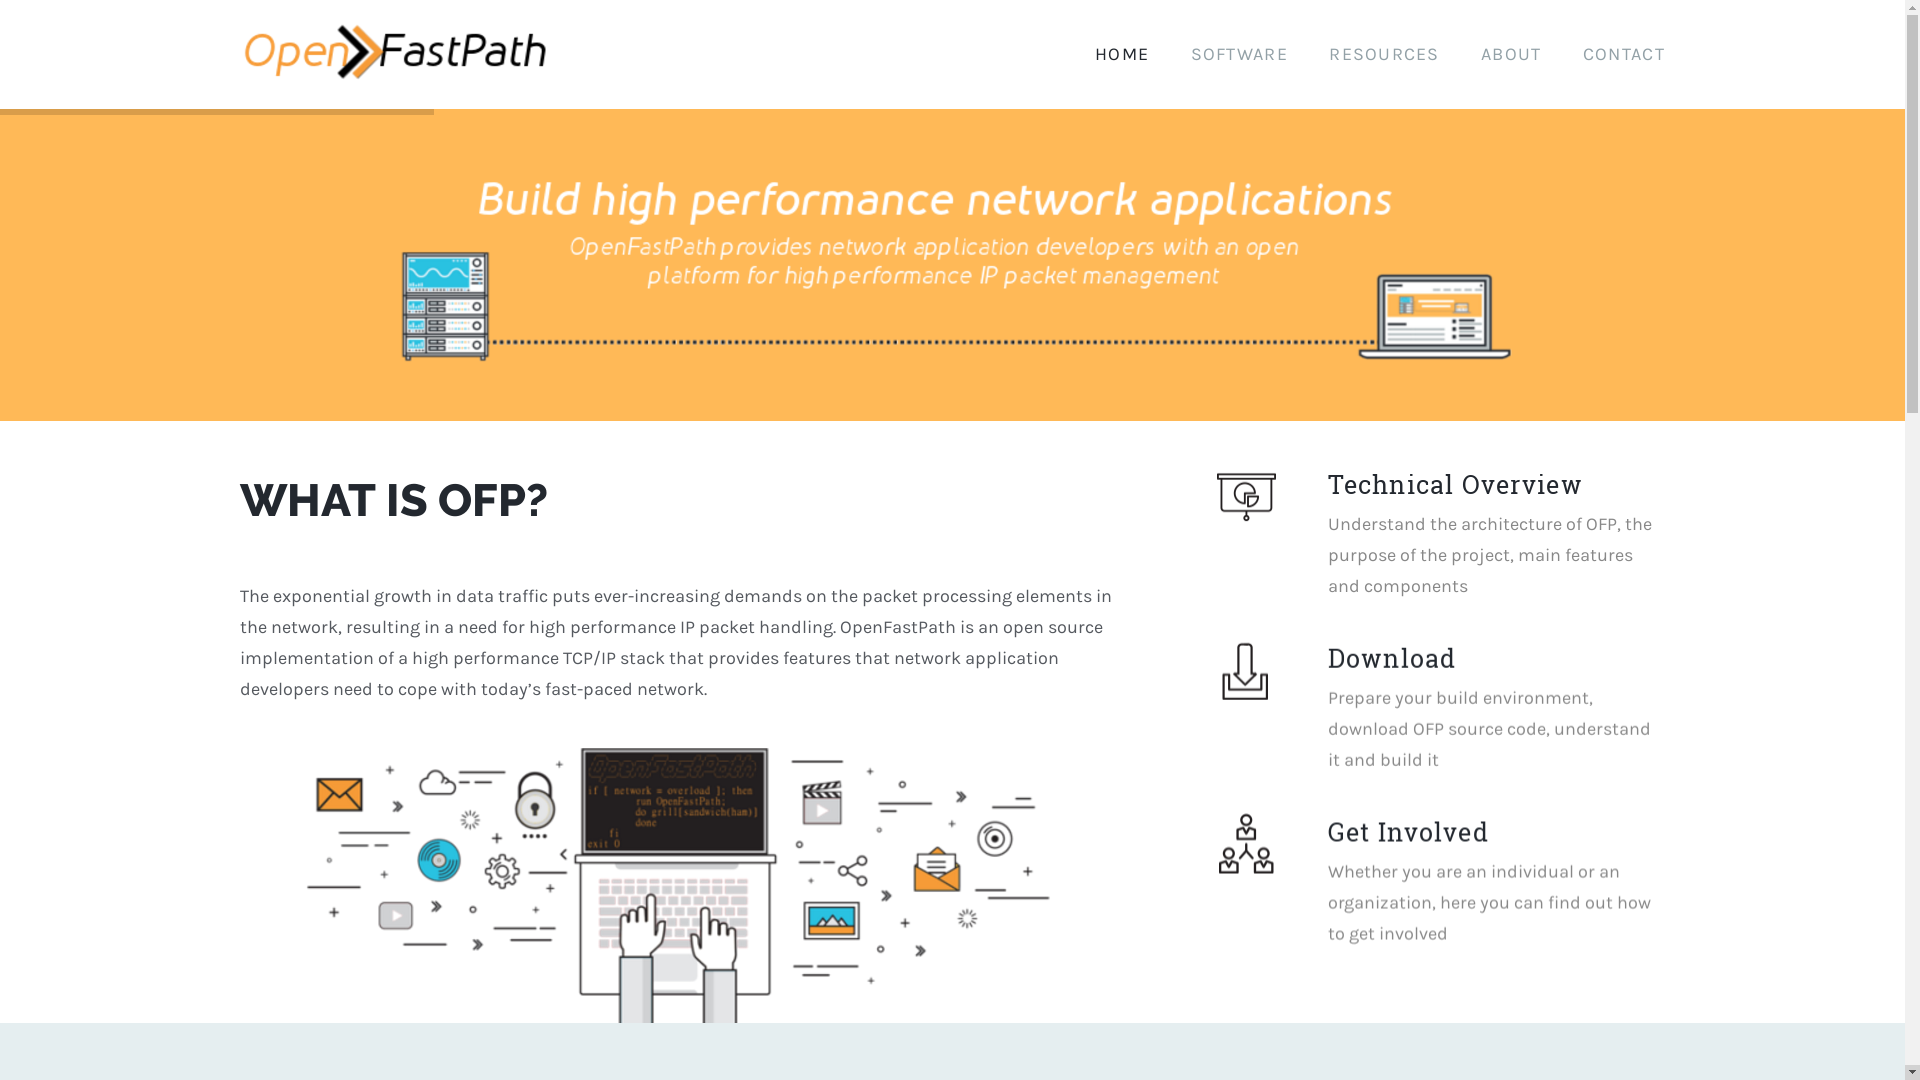
\includegraphics[keepaspectratio=true,height=1.10\textheight,width=1.00\textwidth,angle=0]{www-openfastpath.png}
 \caption{OpenFastPath Website}
 \label{fig:www-openfastpath}
\end{figure}


\begin{itemize}
 \item Website: \\ \url{http://www.openfastpath.org/}
\end{itemize}


``OpenFastPath is an open source implementation of a high performance TCP/IP stack that provides features that network application developers need to cope with today’s fast-paced network.''


\subsection{Open vSwitch}
\begin{figure}[h!]
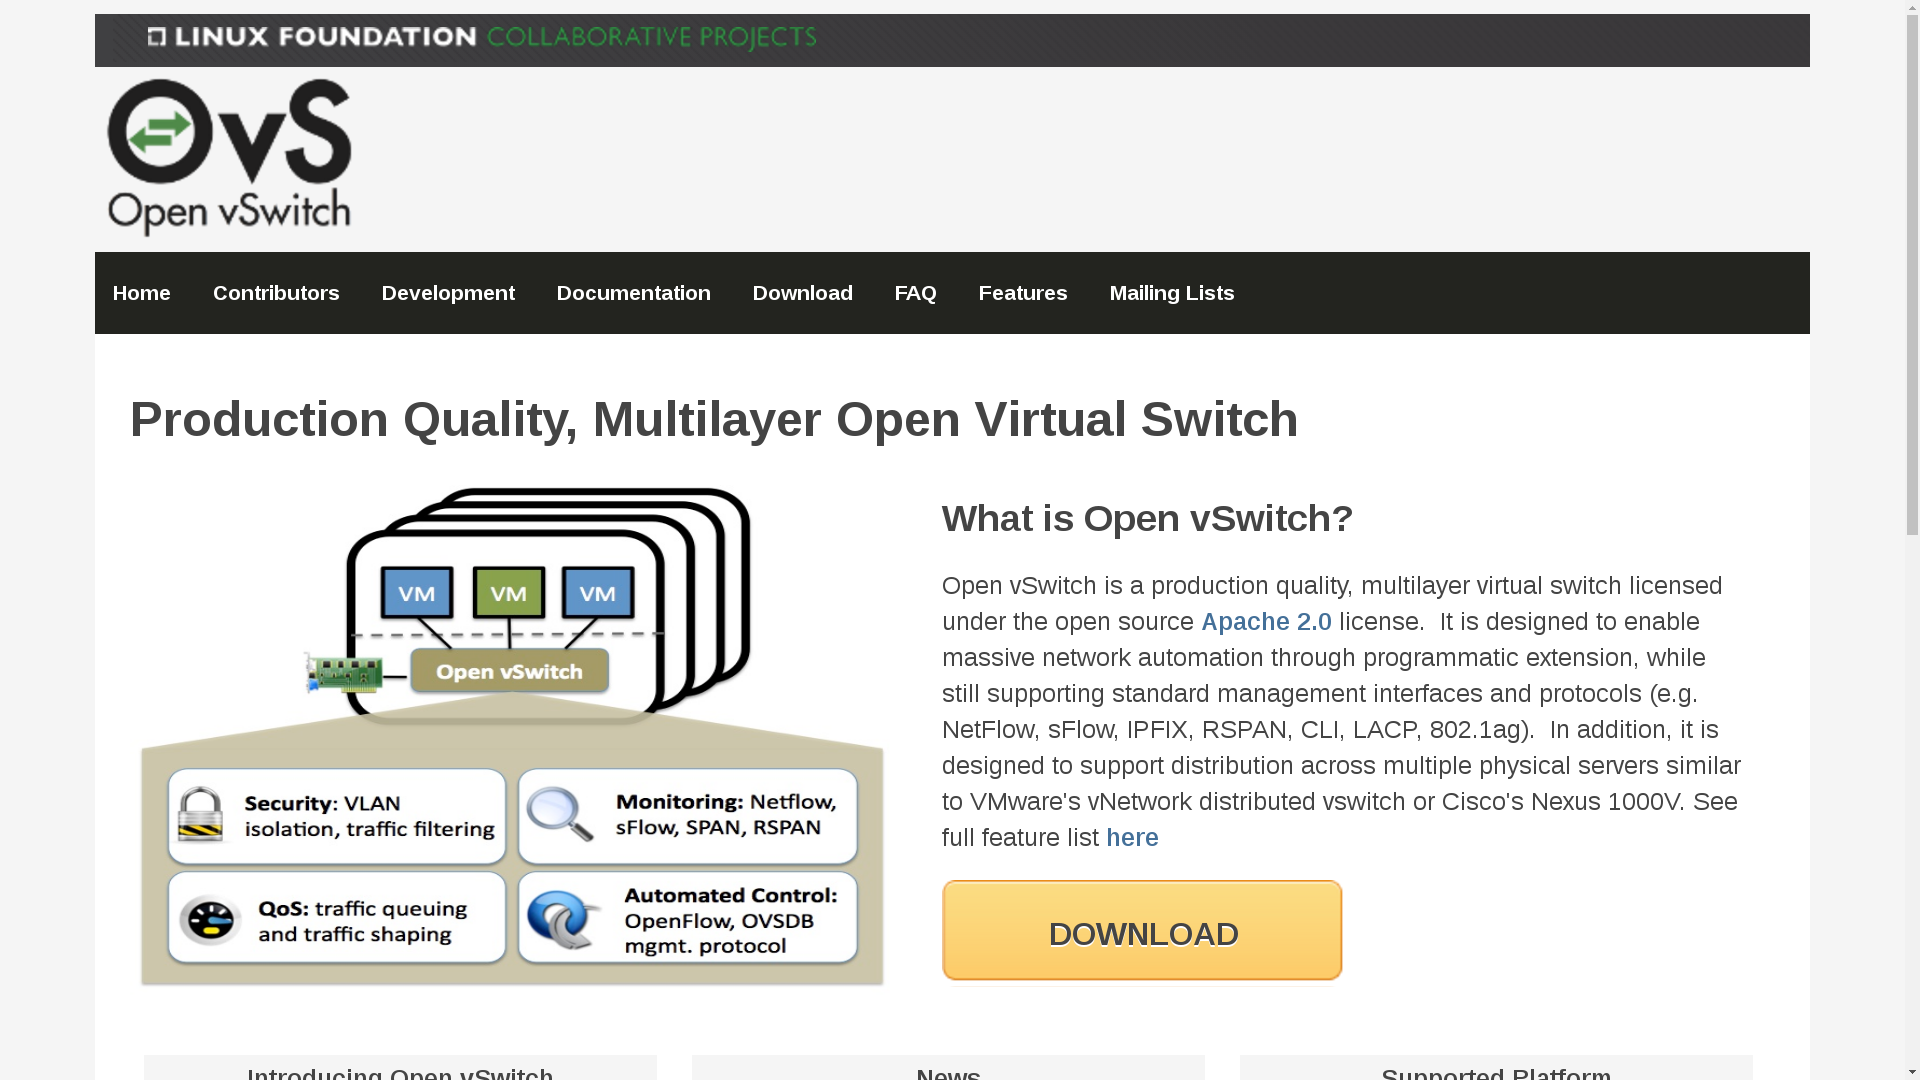
\includegraphics[keepaspectratio=true,height=1.10\textheight,width=1.00\textwidth,angle=0]{www-openvswitch.png}
 \caption{Open vSwitch Website}
 \label{fig:www-openvswitch}
\end{figure}


\begin{itemize}
 \item Website: \\ \url{http://openvswitch.org/}
 \item Linux Foundation Project.
 \item In Debian.
\end{itemize}


``Open vSwitch is a production quality, multilayer virtual switch licensed under the open source Apache 2.0 license.  It is designed to enable massive network automation through programmatic extension, while still supporting standard management interfaces and protocols (e.g. NetFlow, sFlow, IPFIX, RSPAN, CLI, LACP, 802.1ag).''


\subsection{Big Switch}
\begin{figure}[h!]
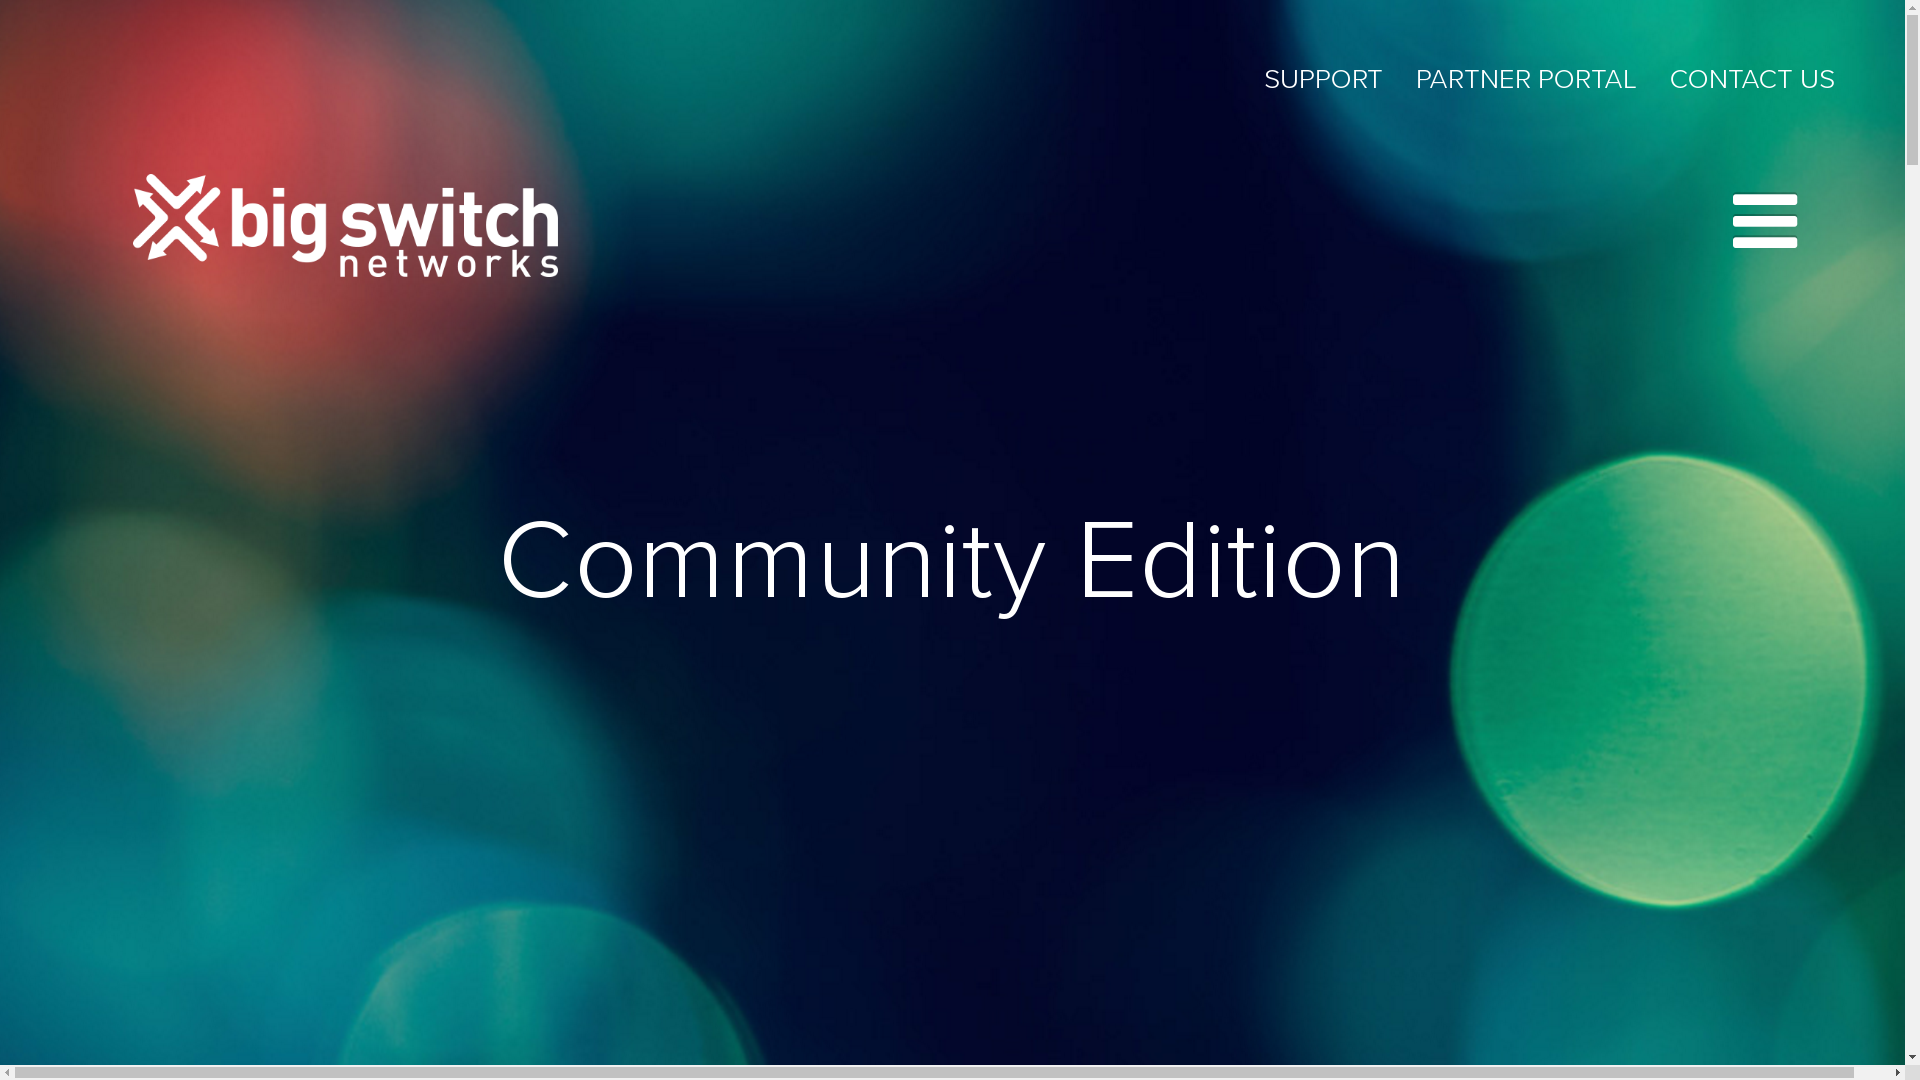
\includegraphics[keepaspectratio=true,height=1.10\textheight,width=1.00\textwidth,angle=0]{www-bigswitch.png}
 \caption{Big Switch Website, no}
 \label{fig:www-bigswitch}
\end{figure}


\begin{itemize}
 \item Website: \\ \url{http://www.bigswitch.com/community-edition}
\end{itemize}


Looks like baitware. Community version is more of a lame demo.
Almost certainly no.


\subsection{Uncategorized Software}
\begin{itemize}
 \item SAI --- Switch Abstraction Interface.
 \item switchdev
\end{itemize}


\url{http://packetpushers.net/sai-and-switchdev-need-to-succeed/}{SAI And Switchdev}
``SAI and switchdev are hardware abstraction models for switching silicon (ASICs). They are the open source frameworks that allow ASICs to be represented in software. This means you can use a Broadcom ASIC the same way as one from Mellanox or Cavium XPliant.''

Microsoft's Azure Cloud Switch (ACS) is ``Debian Jessie + SAI + everything else needed to power Azure (applications like Quagga, and the switch state service based on Redis).'' So their high end switching gear is based on free software, including Quagga and Redis...


\section{Hardware}
Hardware, on which to place free software.


\subsection{Edge-Core}
\begin{figure}[h!]
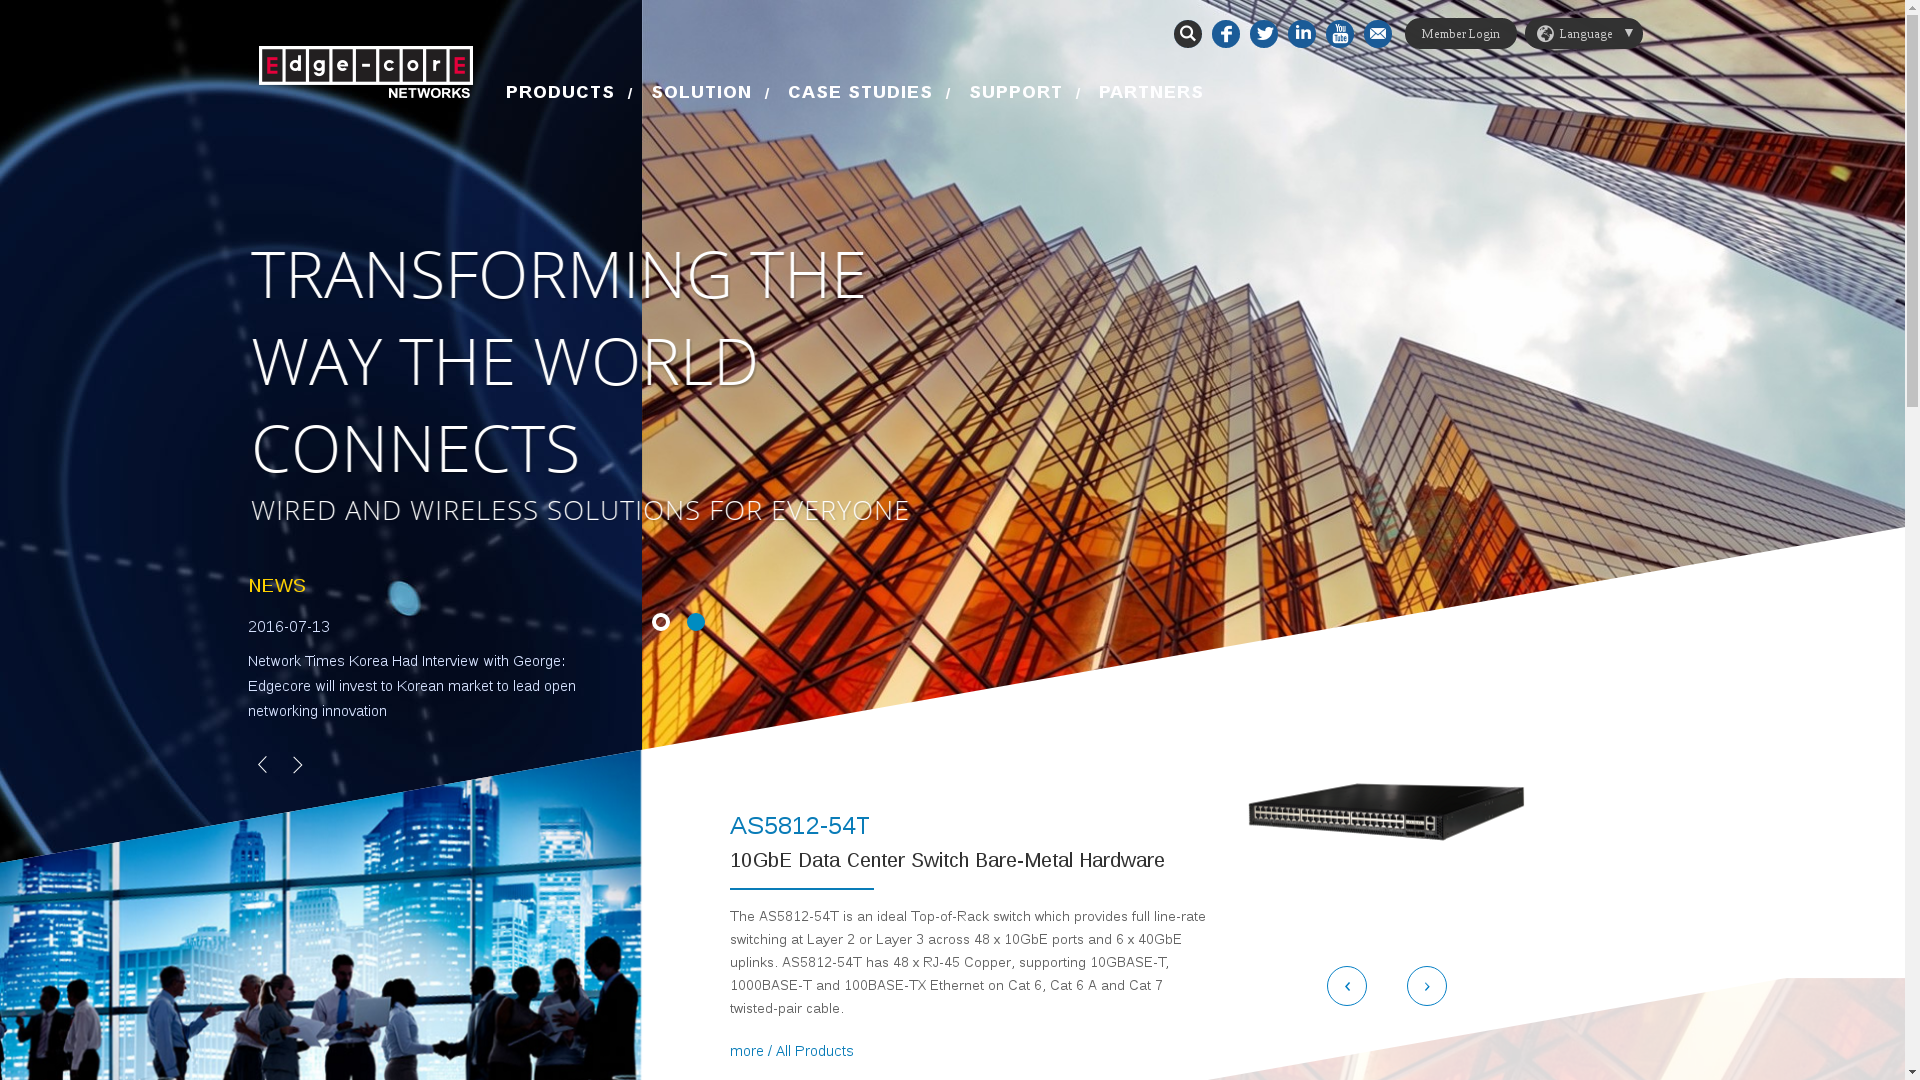
\includegraphics[keepaspectratio=true,height=1.10\textheight,width=1.00\textwidth,angle=0]{www-edge-core.png}
 \caption{Edge-core Website}
 \label{fig:www-edge-core}
\end{figure}


\begin{itemize}
 \item Edge-Core --- Owned by Accton \\ \url{http://www.edge-core.com/}
 \item All Broadcom?
\end{itemize}


\subsection{Dell}
\begin{itemize}
 \item Website: \\ \url{http://dell.com/}
\end{itemize}

Dell makes some bare metal switches that are ONIE compatible.


\subsection{Netberg}
\begin{figure}[h!]
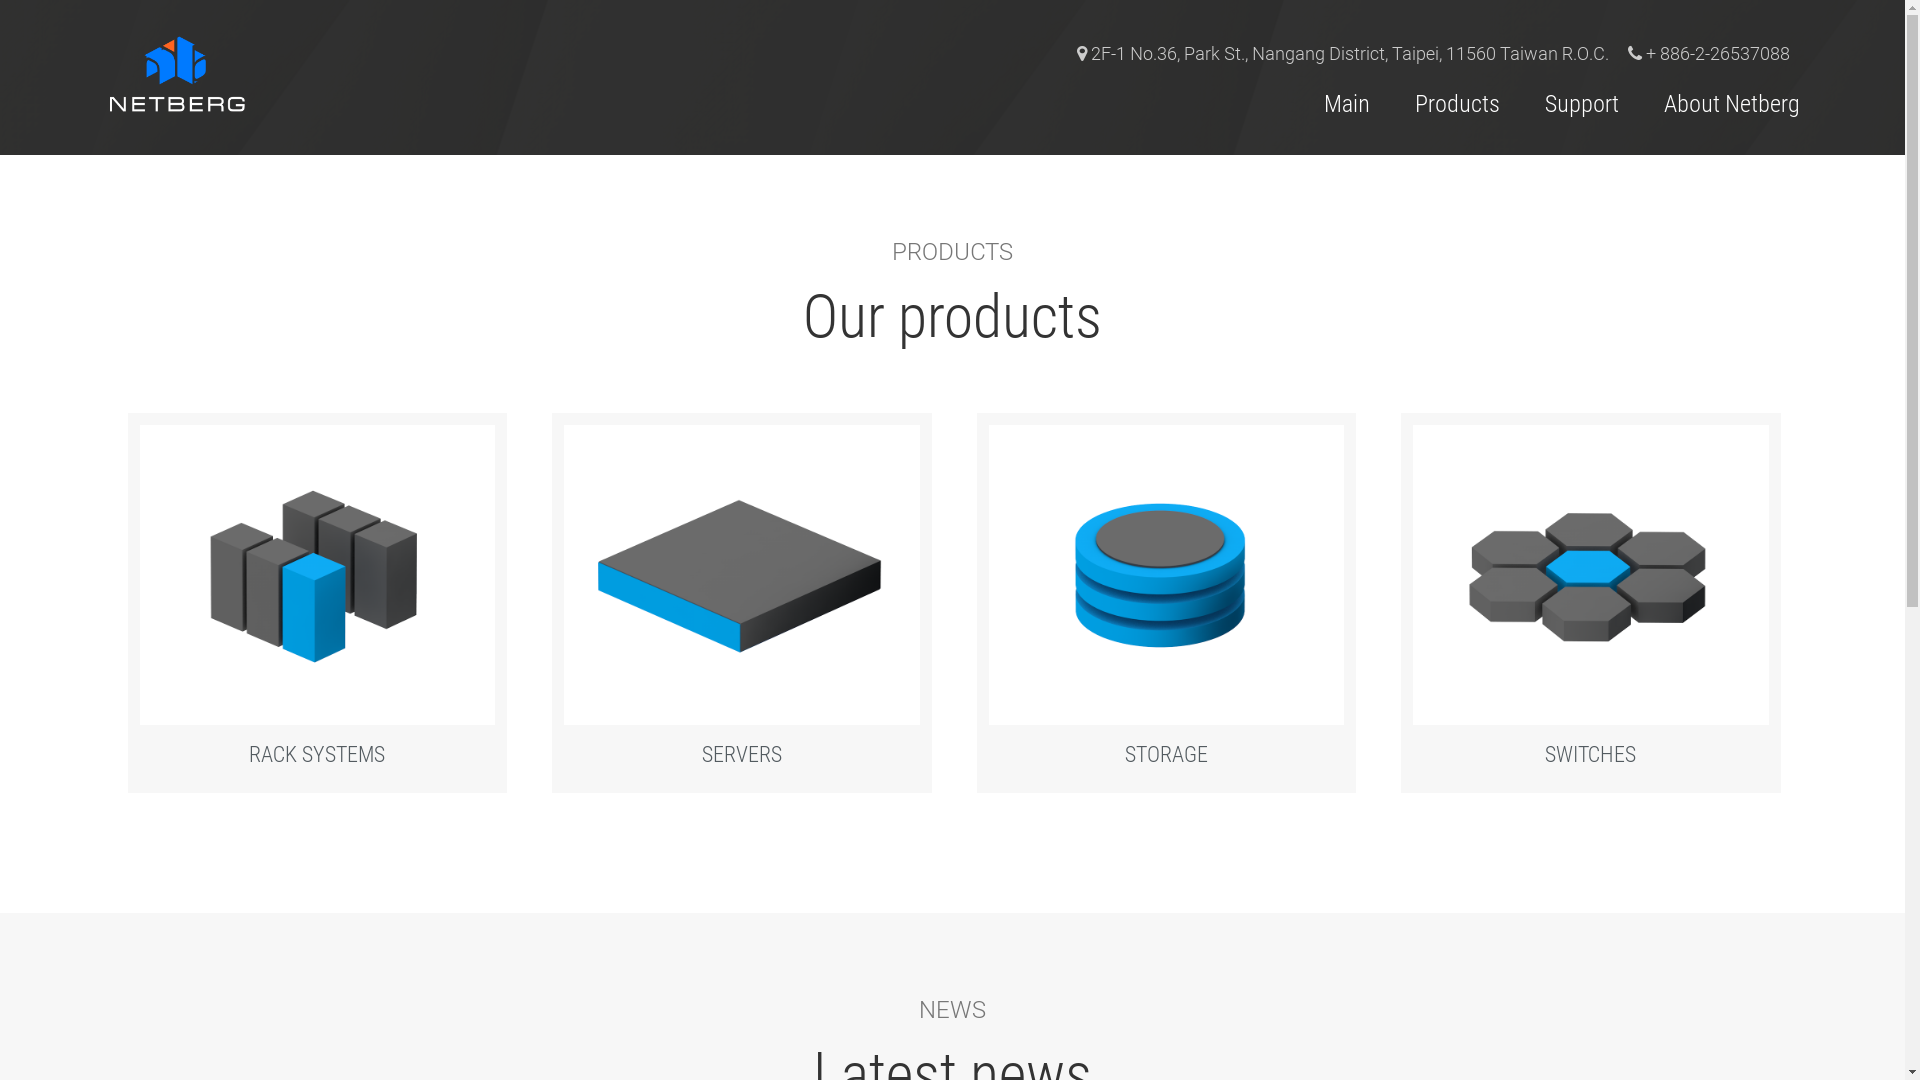
\includegraphics[keepaspectratio=true,height=1.10\textheight,width=1.00\textwidth,angle=0]{www-netberg.png}
 \caption{Netberg Website}
 \label{fig:www-netberg}
\end{figure}


\begin{itemize}
 \item Website: \\ \url{http://netbergtw.com/}
\end{itemize}


Netberg may be the manufacturer of some pfSense branded hardware.


Appears to be...Broadcom based...


\subsection{Quanta}
\begin{figure}[h!]
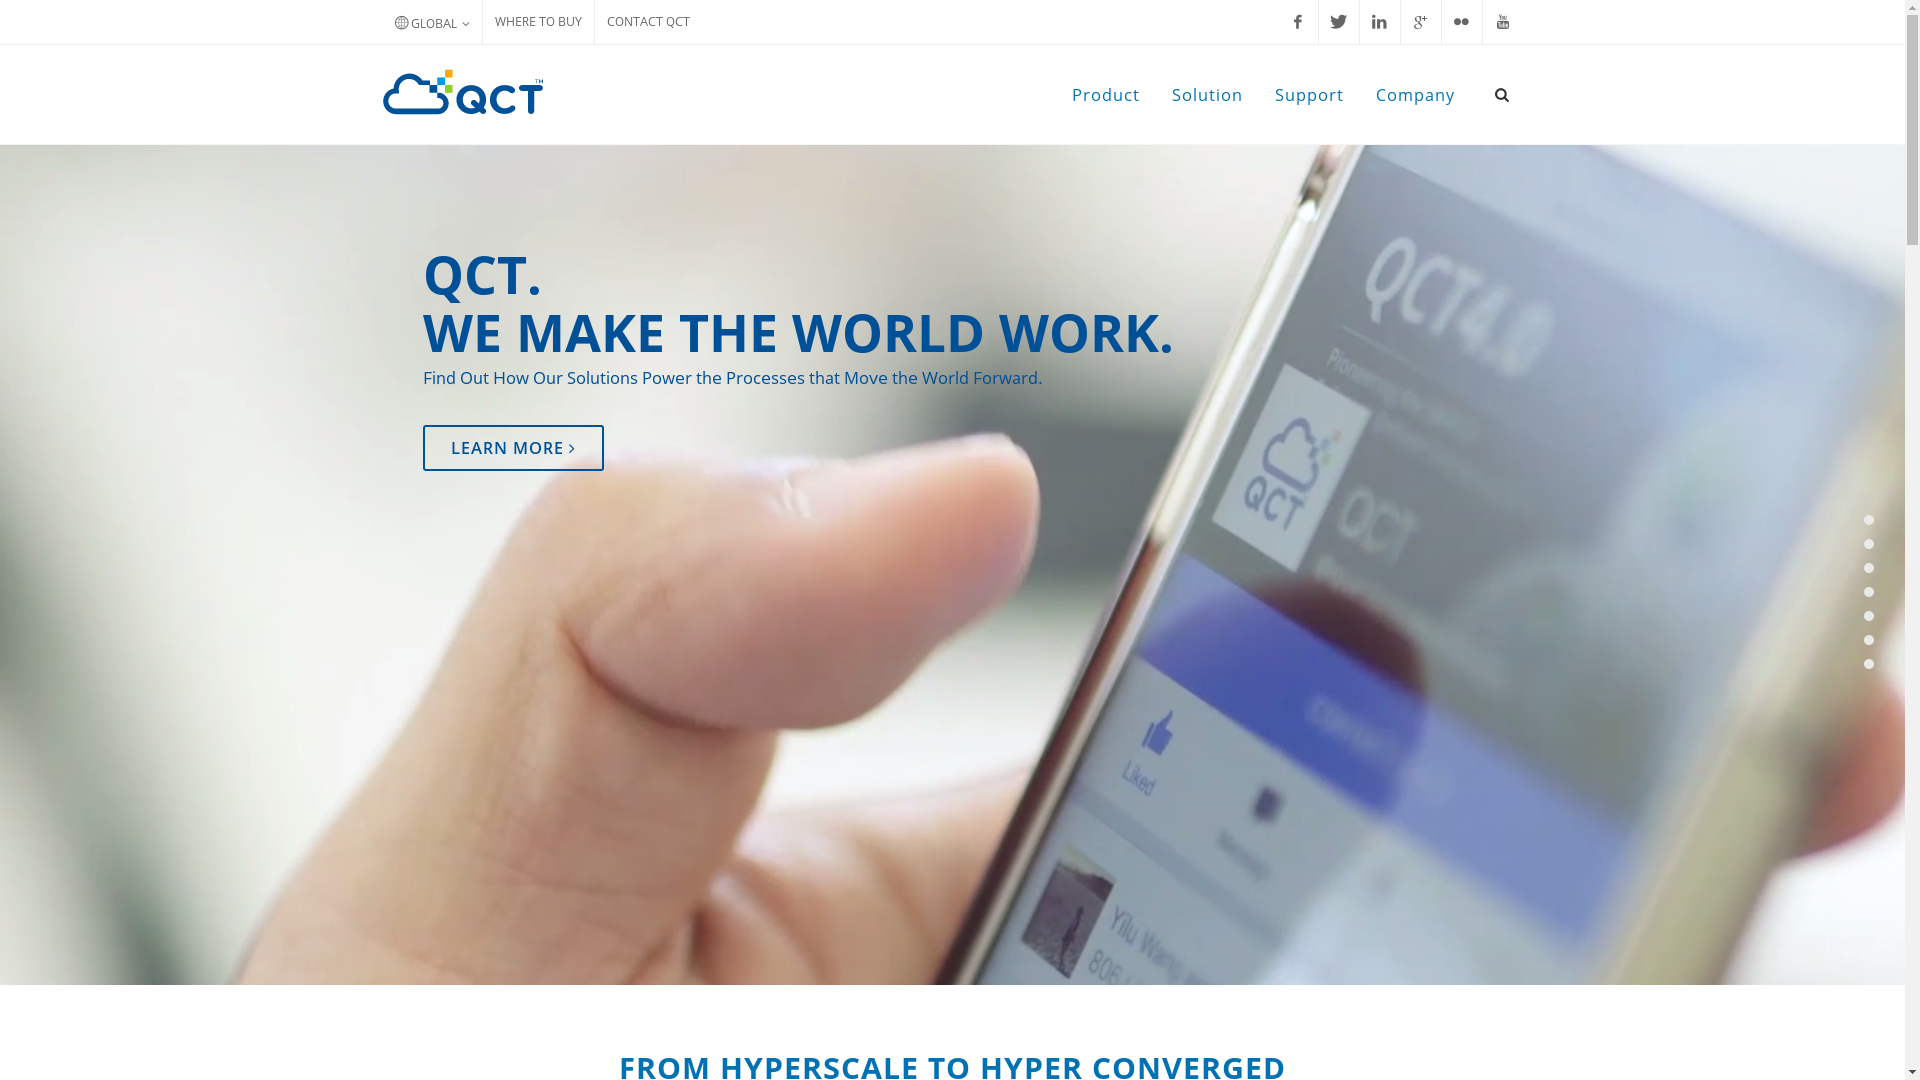
\includegraphics[keepaspectratio=true,height=1.10\textheight,width=1.00\textwidth,angle=0]{www-quanta.png}
 \caption{Quanta Website}
 \label{fig:www-quanta}
\end{figure}


\begin{itemize}
 \item Website: \\ \url{http://www.qct.io/}
 \item Sells "Bare Metal Switches (BMS)"
\end{itemize}


Uses...Broadcom.


\subsection{Mellanox}
\begin{figure}[h!]
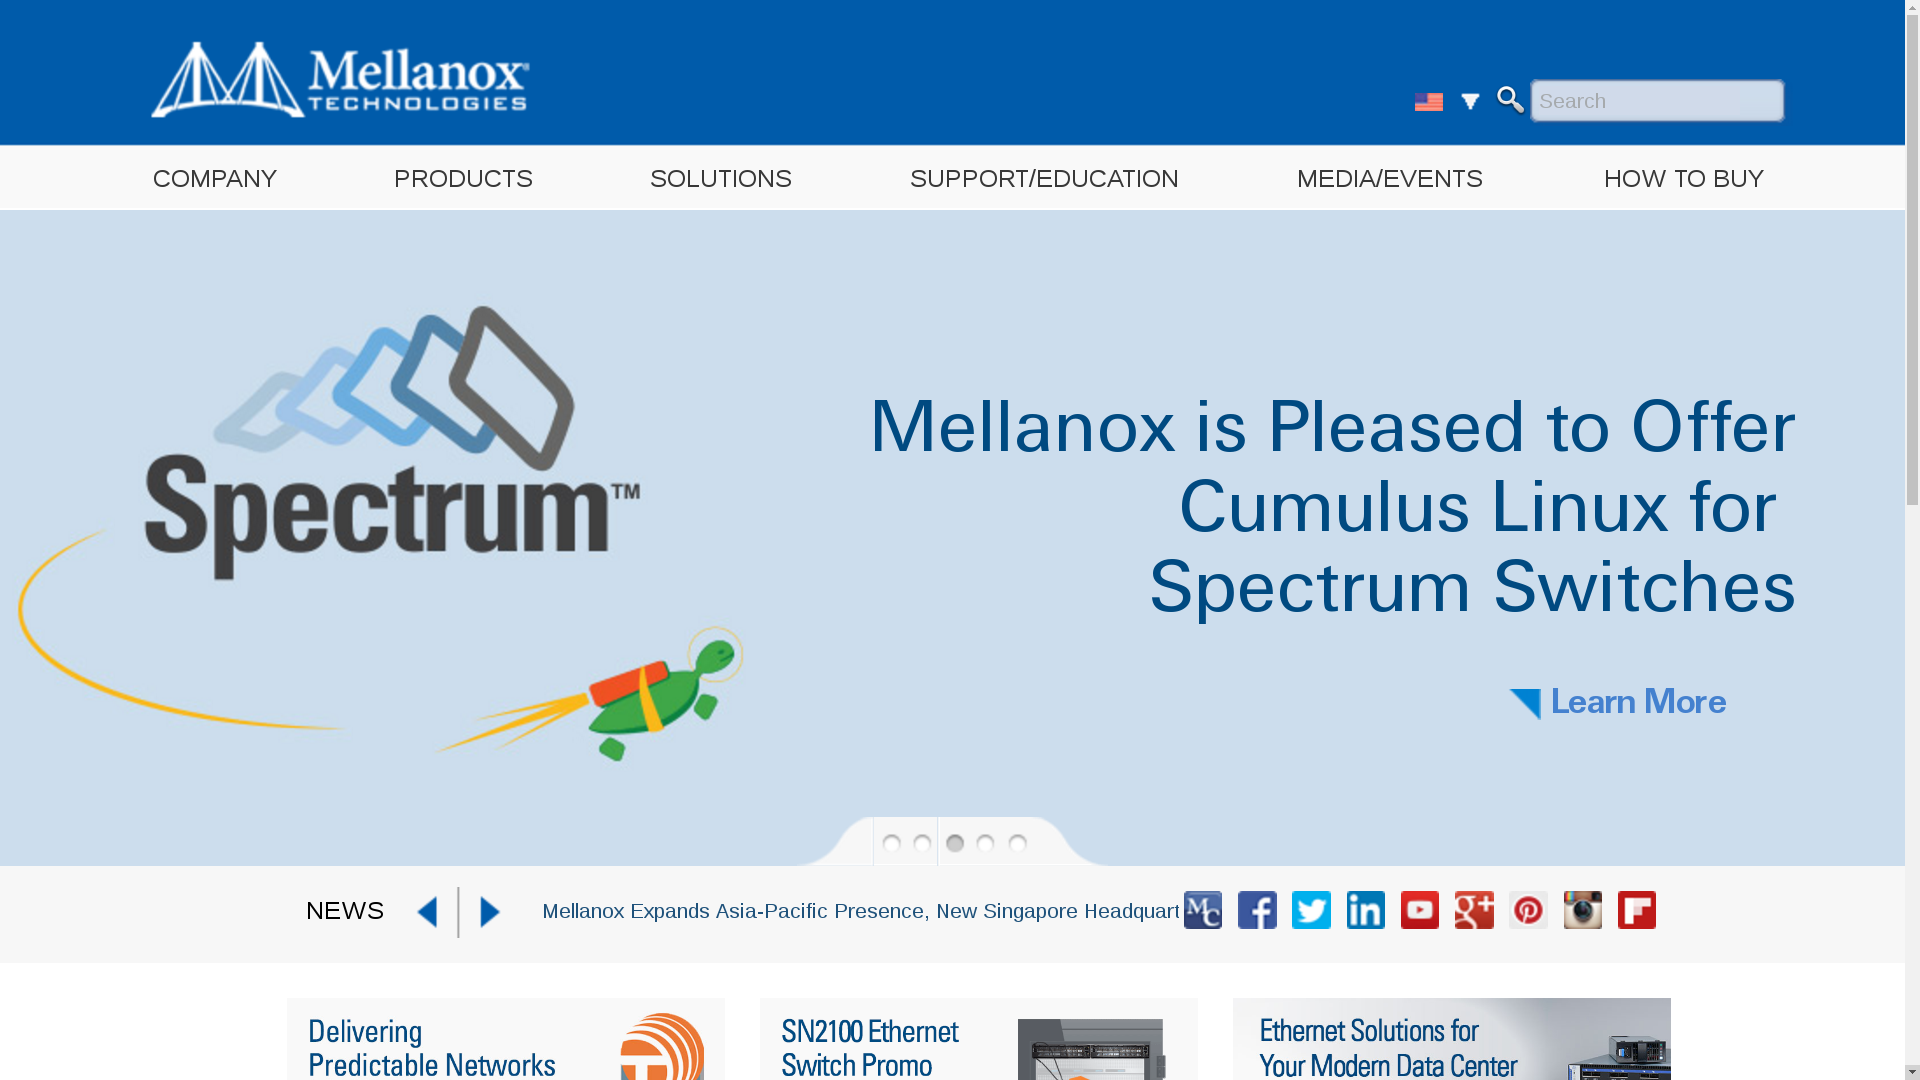
\includegraphics[keepaspectratio=true,height=1.10\textheight,width=1.00\textwidth,angle=0]{www-mellanox.png}
 \caption{Mellanox Website}
 \label{fig:www-mellanox}
\end{figure}


\begin{itemize}
 \item Website: \\ \url{http://www.mellanox.com/}
\end{itemize}


High-end HPC gear, including switches and network cards.


\section{Suppliers}

\subsection{White Box}
\begin{figure}[h!]
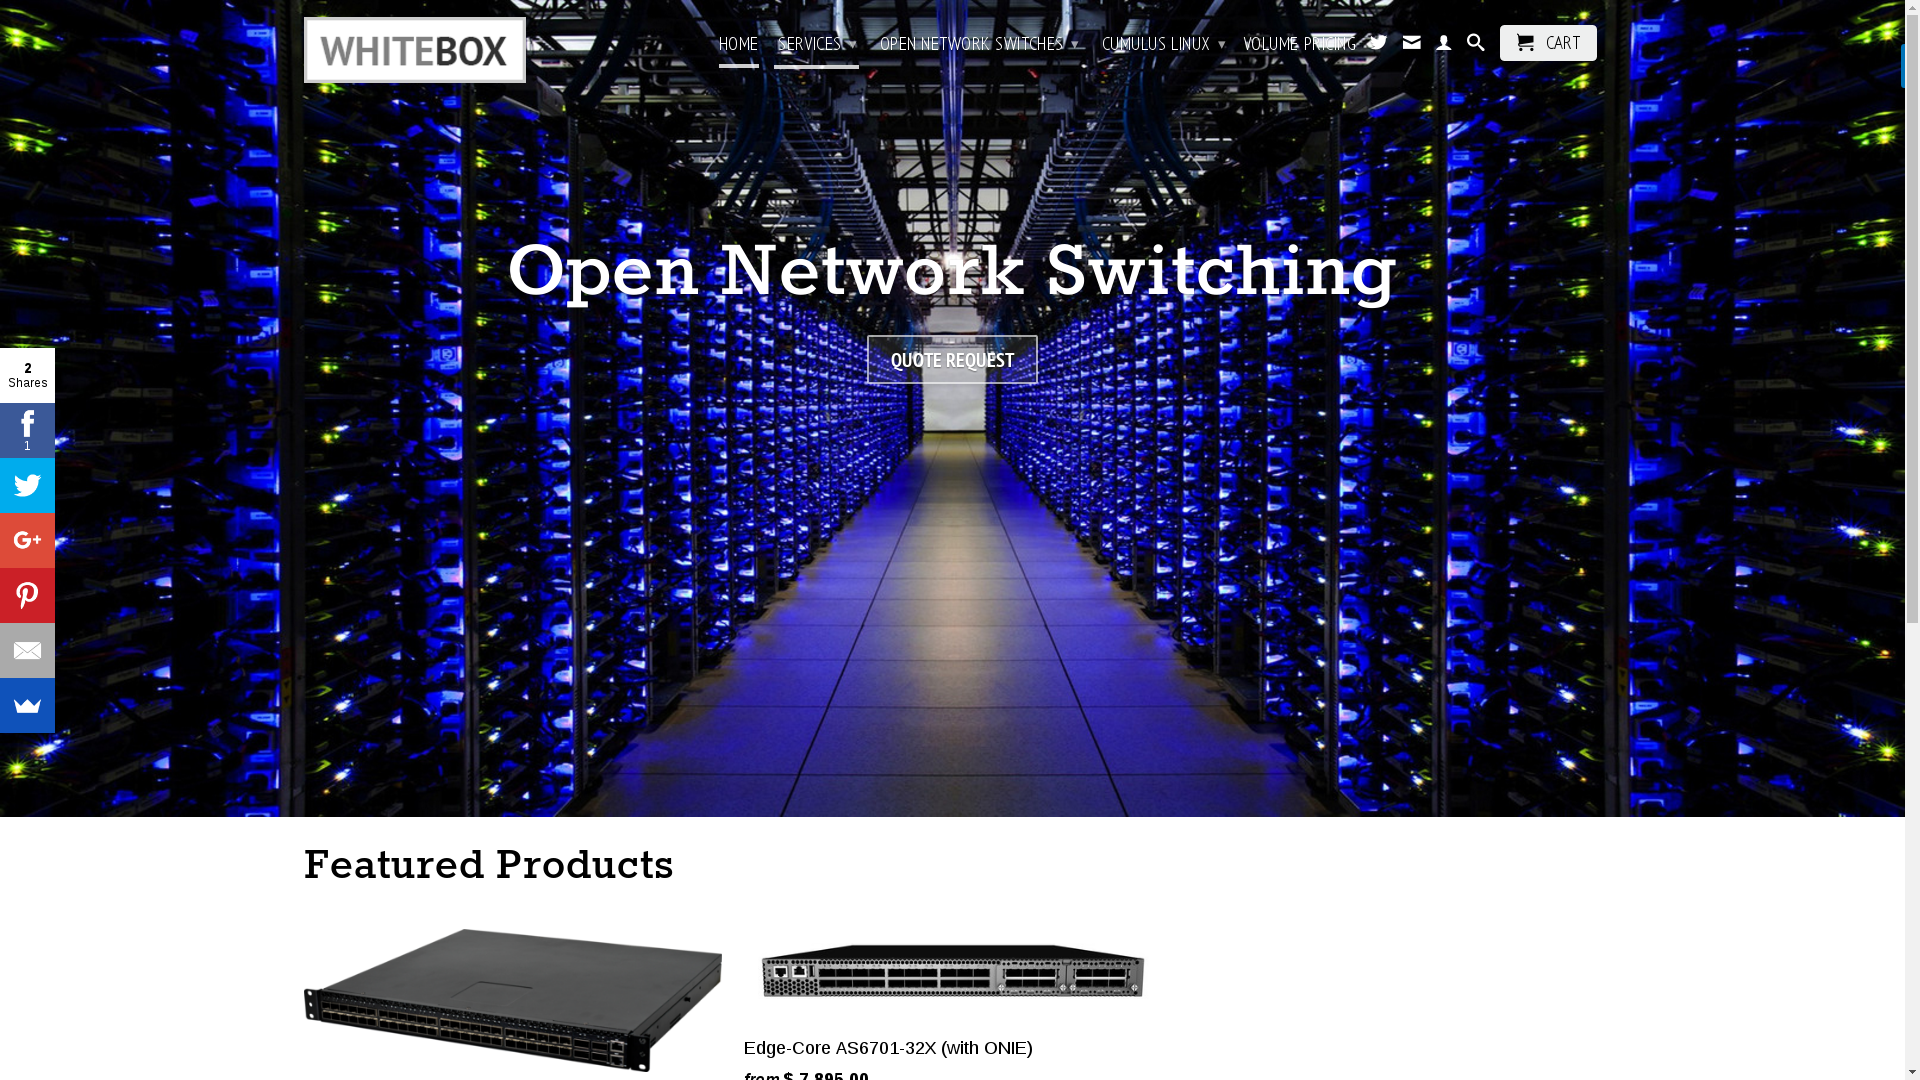
\includegraphics[keepaspectratio=true,height=1.10\textheight,width=1.00\textwidth,angle=0]{www-whitebox.png}
 \caption{Whitebox Website}
 \label{fig:www-whitebox}
\end{figure}


\begin{itemize}
 \item Website: \\ \url{http://whiteboxswitch.com/}
 \item Reseller of open switches.
\end{itemize}


1 Gig-e switches available:
\begin{itemize}
 \item Edge-Core AS4600-54T
 \item Quanta T1048-LB9
\end{itemize}


10 Gig-e switches available:
\begin{itemize}
 \item Edge-Core AS5610-52X (with ONIE)
 \item QuantaMesh BMS T3048-LY2R (with ONIE)
\end{itemize}


40 Gig-e switches available:
\begin{itemize}
 \item Edge-Core AS6701-32X (with ONIE)
 \item QuantaMesh BMS T5032-LY6 (with ONIE)
\end{itemize}


These likely all.have.broadcom.


\subsection{Bare Metal Switches}
\begin{figure}[h!]
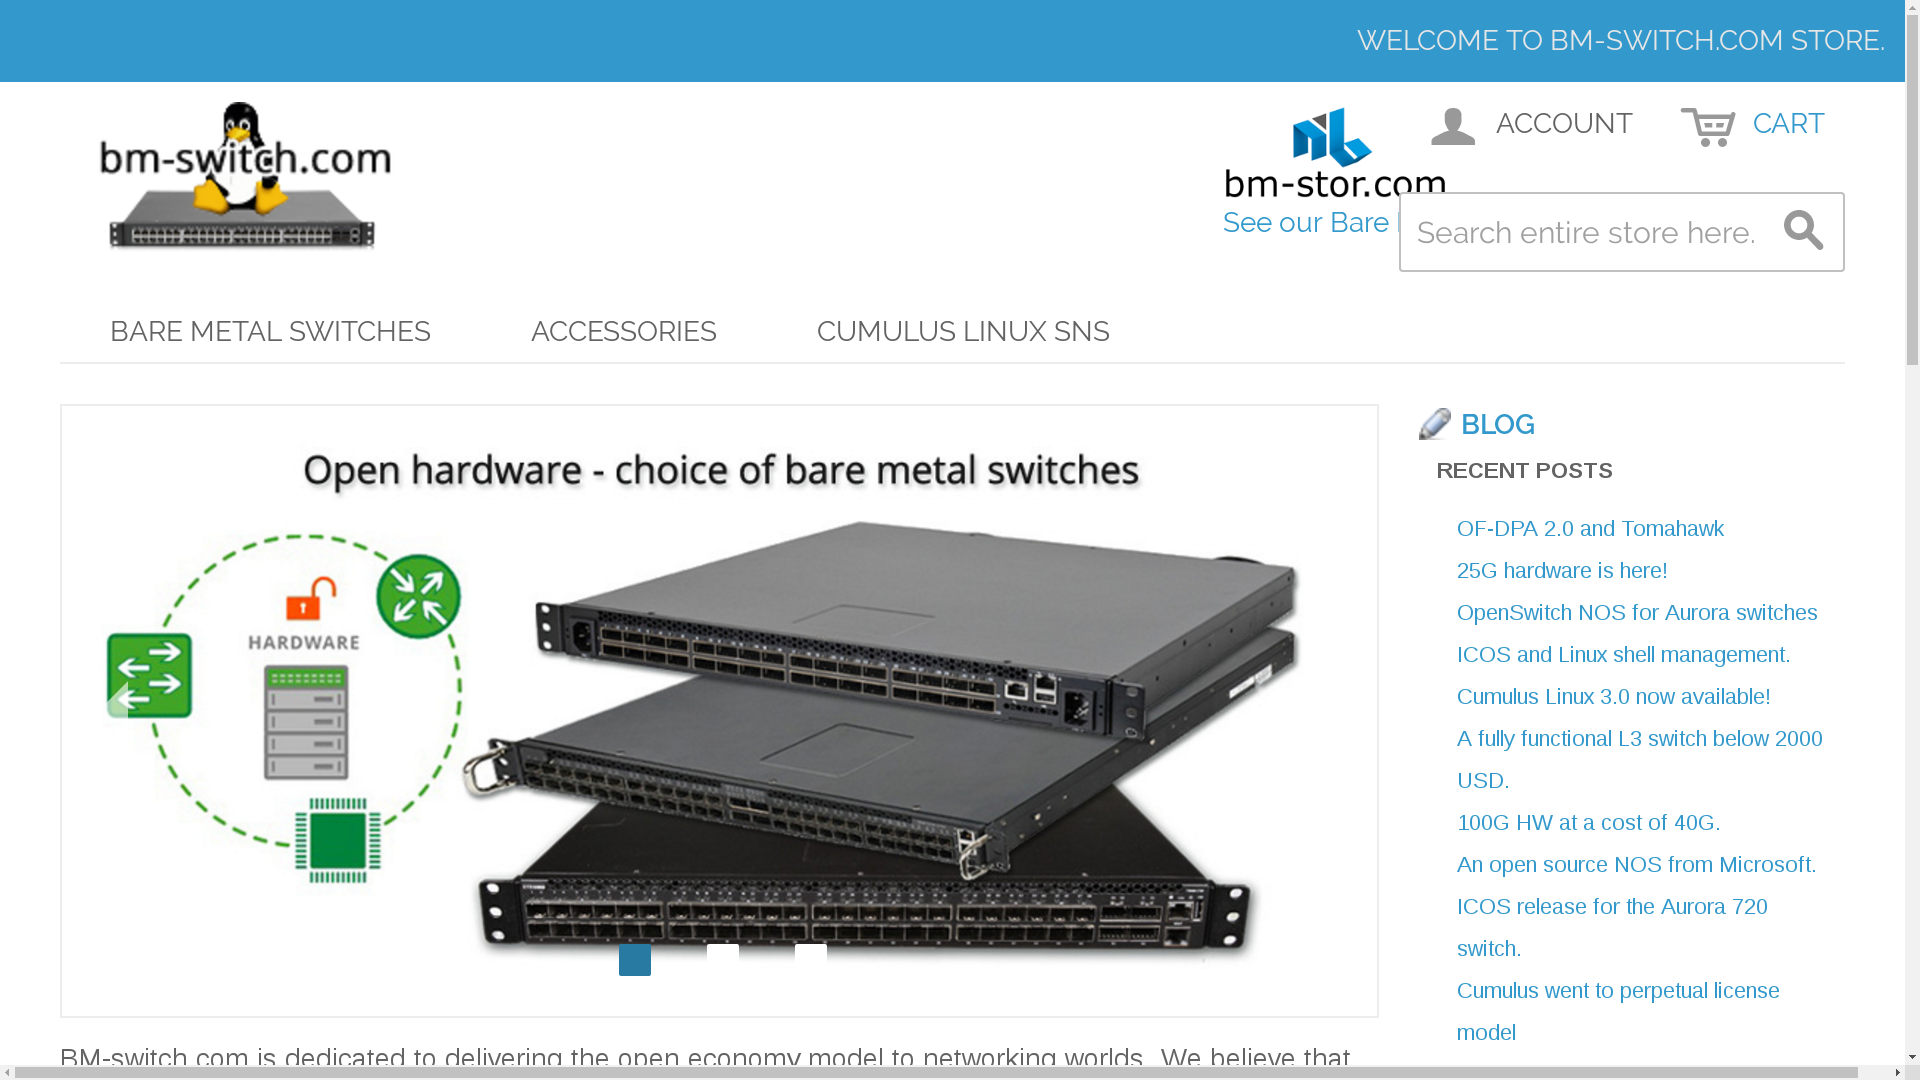
\includegraphics[keepaspectratio=true,height=1.10\textheight,width=1.00\textwidth,angle=0]{www-bm-switch.png}
 \caption{Bare Metal Switches Website}
 \label{fig:www-bm-switch}
\end{figure}


\begin{itemize}
 \item Website: \\ \url{https://bm-switch.com/}
 \item Reseller of open switches.
\end{itemize}


1 Gig-e switches:
\begin{itemize}
 \item Edge-Core AS4600-54T
 \item Edge-Core AS4610-54T (HPE Altoline 6900)
 \item Quanta T1048-LB9
 \item Netberg Aurora 220
\end{itemize}


10 Gig-e switches:
\begin{itemize}
 \item Edge-Core AS5610-52X
 \item Edge-Core AS5710-54X
 \item Edge-Core AS5712-54X (HPE Altoline 6920)
 \item Quanta T3048-LY2
 \item Quanta T3048-LY2R
 \item Quanta T3048-LY8
 \item Quanta T3048-LY9
\end{itemize}


25 Gig-e switches:
\begin{itemize}
 \item Netberg Aurora 620
\end{itemize}


40 Gig-e switches:
\begin{itemize}
 \item Edge-Core AS6700-32X
 \item Edge-Core AS6701-32X
 \item Edge-Core AS6712-32X (HPE Altoline 6940)
 \item Quanta T5032-LY6
\end{itemize}


100 Gig-e switches:
\begin{itemize}
 \item Netberg Aurora 720
 \item Edge-Core AS7712-32X (HPE Altoline 6960)
\end{itemize}


All of the switches from Bare Metal Switches appear to use Broadcom ASICs.
Broadcom contributed code to OpenCompute, which is an ``Open Source'' project,
but what they include in github has a clearly non-free license:


\url{https://github.com/Broadcom-Switch/OpenNSL/blob/master/Legal/LICENSE-Adv}


``Licensee will not:
Sell, rent, lease, distribute, sublicense, assign, or otherwise transfer
(including by loan or gift) the Code''.


I am disinclined to use Broadcom firmware:


\url{https://web.archive.org/web/20080411030140/http://jebba.blagblagblag.org/?p=244}


The switches they carry have a variety of CPUs:
Freescale P2020 (PPC), Intel Atom, ARM.


The switches can run a variety of OSs, many non-free. They likely need non-free
Broadcom firmware regardless of the OS (including ONL).


\begin{itemize}
 \item OpenNSL -- Broadcom chipsets. Accton. Github archive has proprietary
   license (LICENSE-Adv = non-free).
 \item OF-DPA -- From Broadcom.
 \item SAI 
\end{itemize}


\subsection{Colfax Direct}
\begin{figure}[h!]
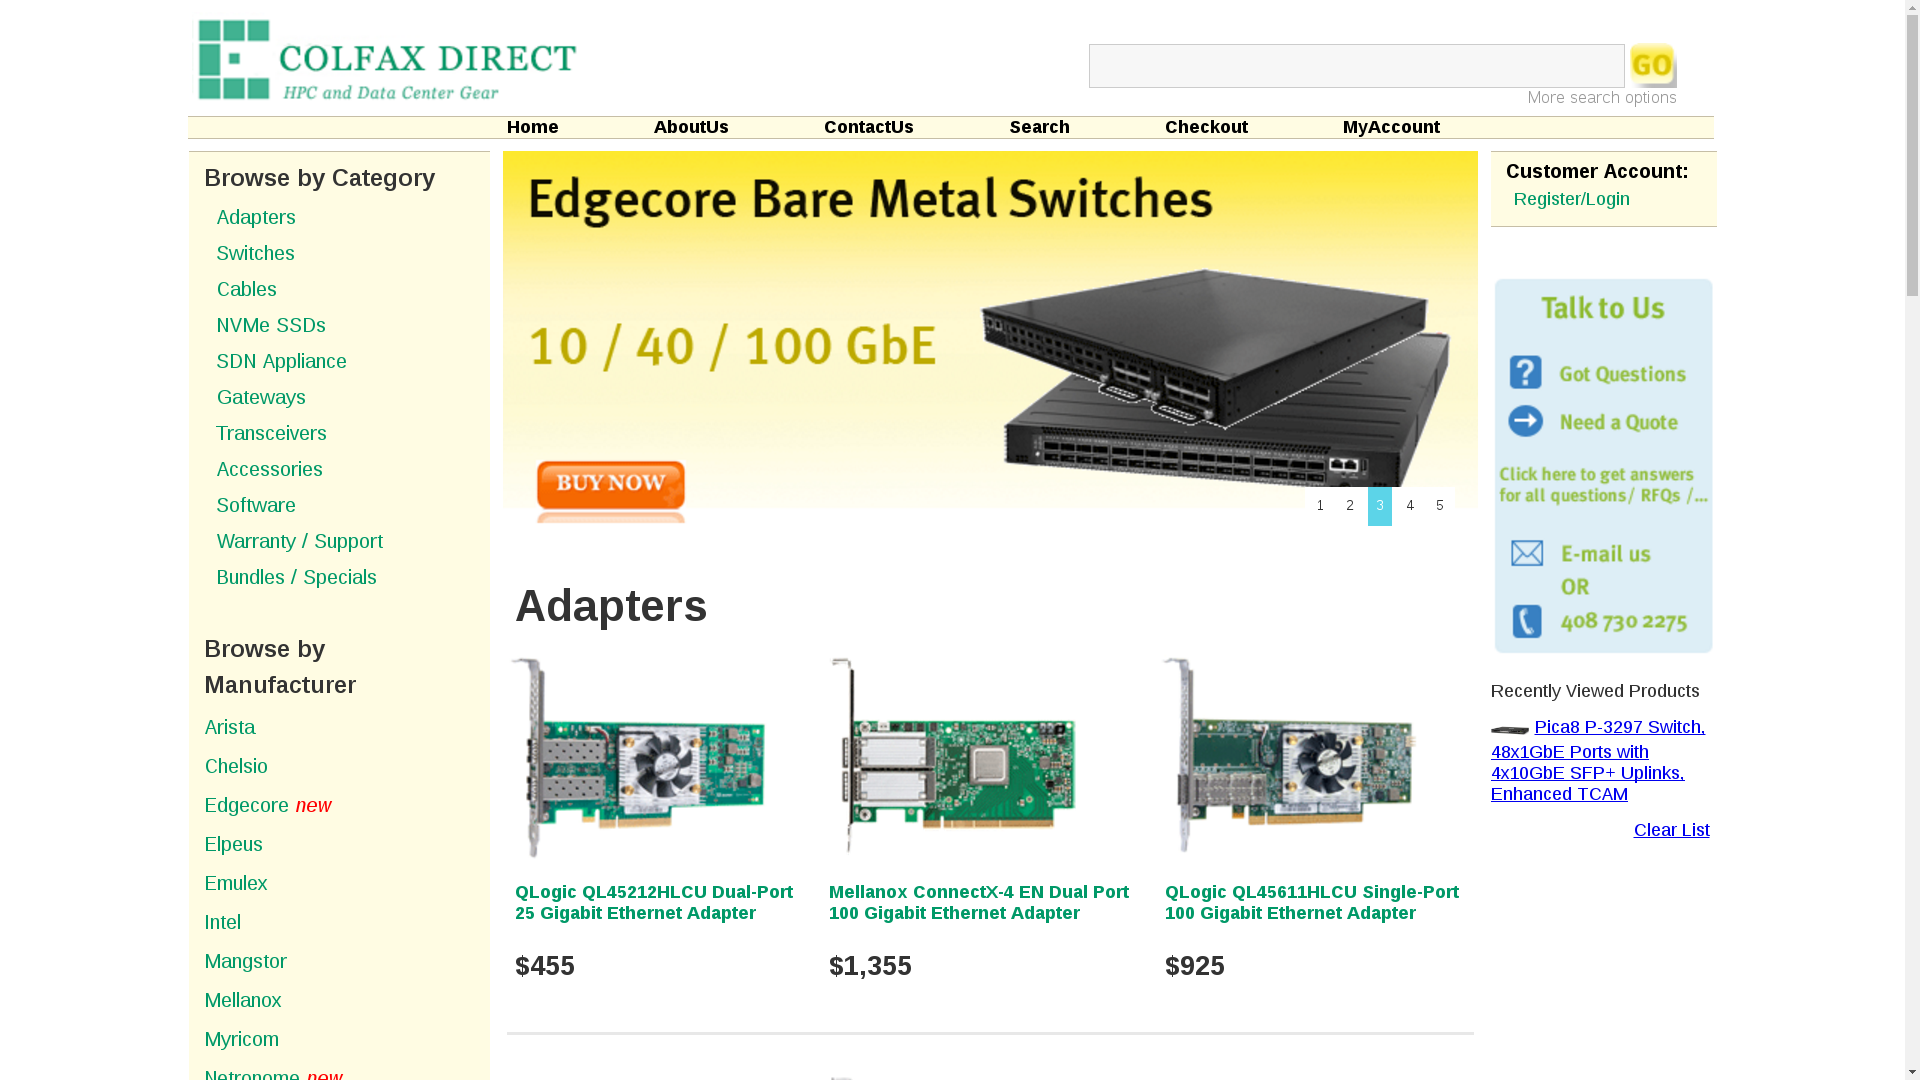
\includegraphics[keepaspectratio=true,height=1.10\textheight,width=1.00\textwidth,angle=0]{www-colfax.png}
 \caption{Colfax Direct Website}
 \label{fig:www-colfax}
\end{figure}


\begin{itemize}
 \item Website: \\ \url{http://www.colfaxdirect.com/}
 \item Switches: \\ \url{http://www.colfaxdirect.com/store/pc/viewCategories.asp?idCategory=7}
\end{itemize}


Colfax Direct sells a variety of HPC gear, including bare metal switches.
They have network cards and other bits.


\subsection{Penguin Computing}
\begin{itemize}
 \item Website: \\ \url{http://www.penguincomputing.com/}
\end{itemize}


Slow manual order/quote process.

